\documentclass[UTF8, a4paper, 12pt]{ctexart}

%=================== 宏包引用 ===================
\usepackage{geometry}           % 页面布局
\usepackage{amsfonts, amsmath, amssymb, amsthm} % 数学公式符号
\usepackage{graphicx}           % 图片插入
\usepackage{float}              % 浮动体控制
\usepackage{caption}            % 图表标题
\usepackage{fancyhdr}           % 页眉页脚
\usepackage{listings}           % 代码抄录
\usepackage{xcolor}             % 颜色支持
\usepackage{booktabs}           % 三线表
\usepackage{hyperref}           % 超链接与书签
% 在导言区添加 TikZ 支持
\usepackage{tikz}
\usepackage{diagbox} % 用于绘制斜线表头
\usepackage{multirow}
\usetikzlibrary{shapes, arrows, positioning, calc}

%=================== 页面设置 ===================
\geometry{left=2.5cm, right=2.5cm, top=2.5cm, bottom=2.5cm}

%=================== 标题格式修正 ===================
% 强制一级标题左对齐，取消默认的居中
\ctexset{
    section = {
        format = \Large\bfseries\raggedright, % 左对齐
        aftername = \hspace{1em} 
    }
}

%=================== 代码高亮设置 ===================
\definecolor{codegreen}{rgb}{0,0.6,0}
\definecolor{codegray}{rgb}{0.5,0.5,0.5}
\definecolor{codepurple}{rgb}{0.58,0,0.82}
\definecolor{backcolour}{rgb}{0.95,0.95,0.92}

\lstset{
    language=Matlab,
    backgroundcolor=\color{backcolour},   
    commentstyle=\color{codegreen},
    keywordstyle=\color{blue},
    numberstyle=\tiny\color{codegray},
    stringstyle=\color{codepurple},
    basicstyle=\ttfamily\footnotesize,
    breakatwhitespace=false,         
    breaklines=true,                 
    captionpos=b,                    
    keepspaces=true,                 
    numbers=left,                    
    numbersep=5pt,                  
    showspaces=false,                
    showstringspaces=false,
    showtabs=false,                  
    tabsize=2,
    frame=single
}

%=================== 常用数学命令 ===================
\newcommand{\dif}{\mathrm{d}}
\newcommand{\avg}[1]{\left\langle #1 \right\rangle}
\newcommand{\difFrac}[2]{\frac{\dif #1}{\dif #2}}
\newcommand{\pdfFrac}[2]{\frac{\partial #1}{\partial #2}}

%=================== 页眉页脚设置 ===================
\pagestyle{fancy}
\fancyhead{} 
\lhead{郭子昊, 3230104714}
\chead{智能控制技术：大作业}
\rhead{\today}
\cfoot{\thepage}

%=================== 文档开始 ===================
\begin{document}

%------------------- 封面部分 -------------------
\begin{center}
    \vspace*{1cm}
    \huge\bfseries 智能控制技术大作业报告\\[0.5cm]
    \Large —— 基于多策略对比的固定翼无人机纵向非线性控制系统设计与仿真\\[2cm]
    
    \large
    \begin{tabular}{rl}
        \textbf{姓名：} & 郭子昊 \\
        \textbf{学号：} & 3230104714 \\
        \textbf{课程：} & 智能控制技术 \\
        \textbf{日期：} & \today \\
    \end{tabular}
\end{center}
\vspace{2cm}
\thispagestyle{empty}
\newpage
\setcounter{page}{1}

%------------------- 正文部分 -------------------

%=================== 第一部分：问题概述 ===================
\section{问题概述}

\subsection{问题背景}
随着航空航天技术与人工智能的深度融合，固定翼无人机（Fixed-Wing Unmanned Aerial Vehicle, UAV）因其具有巡航速度快、续航时间长、负载能力强等显著优势，在军事侦察、地质勘测、物流运输及灾害救援等领域发挥着不可替代的作用。然而，固定翼无人机的纵向飞行控制系统是一个典型的高阶、非线性、强耦合且欠驱动的复杂动力学系统。

在实际飞行包线内，无人机面临着多重严峻挑战：
\begin{enumerate}
    \item \textbf{严重的动态耦合}：纵向运动涉及飞行速度与飞行高度（或俯仰角）的协同控制。调节升降舵不仅改变姿态，还会引起诱导阻力的变化从而影响速度；反之，调节油门也会通过推力力矩直接干扰俯仰平衡。
    \item \textbf{气动非线性与模型不确定性}：无人机的升力、阻力及俯仰力矩系数随攻角（Angle of Attack）和马赫数呈现高度非线性变化。特别是在大机动飞行或气流分离区域，线性化模型误差巨大。
    \item \textbf{复杂的外部环境干扰}：低空飞行时常遭遇阵风、风切变等突发气流扰动，这对控制系统的抗扰动能力（鲁棒性）提出了极高要求。
\end{enumerate}

传统的线性控制方法（如 PID）通常基于某一平衡点进行小扰动线性化设计，难以在宽包线范围内兼顾动态响应速度与稳态精度。为了探索更高效、更鲁棒的控制方案，本大作业将从智能控制的角度出发，循序渐进地研究模糊控制、神经网络控制及滑模变结构控制在无人机纵向飞行中的应用。

%=================== 第二部分：系统建模 ===================
\section{系统建模}

本大作业的被控对象为固定翼无人机的纵向飞行运动。该模型来源于经典航空控制文献[1]，属于典型的多变量非线性动力学模型。为了真实模拟飞行过程，本节将基于牛顿-欧拉力学体系，建立包含气动非线性特性的状态空间方程。

\subsection{坐标系定义与受力分析}
在研究无人机运动时，我们需要定义两个关键坐标系：
\begin{itemize}
    \item \textbf{机体坐标系 ($O_b x_b y_b z_b$)}：原点位于质心，${x_b}$ 轴指向机头方向，${z_b}$ 轴在对称面内指向机腹。
    \item \textbf{气流坐标系 ($O_w x_w y_w z_w$)}：${x_w}$ 轴沿着速度矢量 $\mathbf{V}$ 的方向。
\end{itemize}

\begin{figure}[H]
    \centering
    % 请确保 figure 文件夹下有 force_model.png 图片
    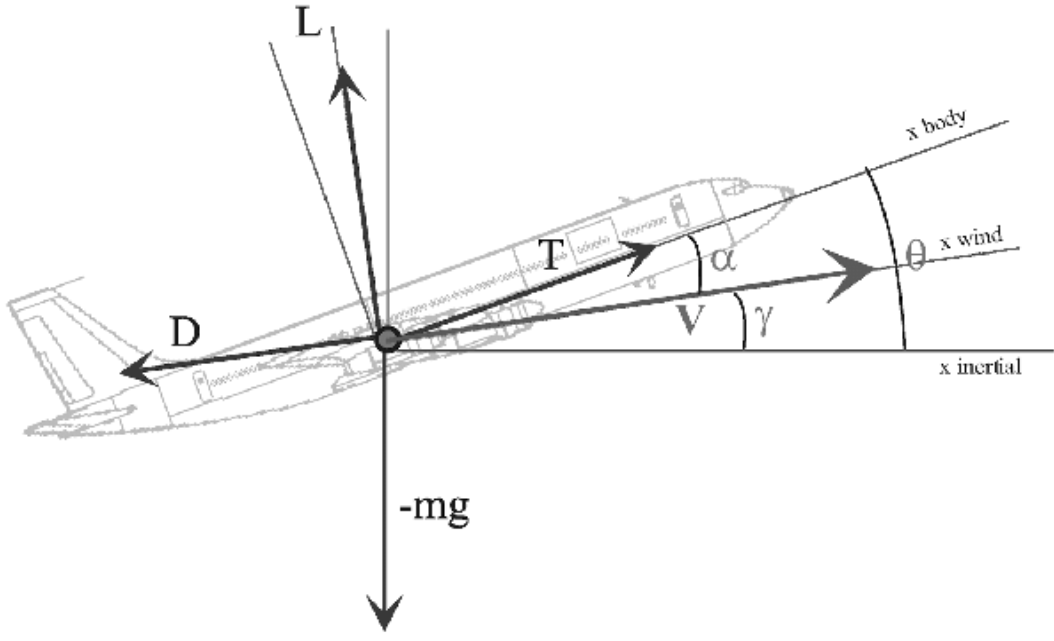
\includegraphics[width=0.7\textwidth]{figure/force_model.png} 
    \caption{固定翼无人机纵向飞行受力分析与坐标系定义}
    \label{fig:forces}
\end{figure}

如图 \ref{fig:forces} 所示，无人机在纵向平面内主要受到四个力的作用：重力 $mg$、发动机推力 $T$、气动升力 $L$ 和气动阻力 $D$。其中，升力 $L$ 垂直于速度矢量，阻力 $D$ 平行于速度矢量反向。

定义关键角度变量如下：
\begin{equation}
    \alpha = \theta - \gamma
\end{equation}
其中，$\theta$ 为俯仰角（机体轴与水平面夹角），$\gamma$ 为航迹角（速度矢量与水平面夹角），$\alpha$ 为攻角（机体轴与速度矢量夹角）。

\subsection{非线性动力学方程推导}
根据牛顿第二定律，在气流坐标系下分解各力，可得速度 $V$ 和航迹角 $\gamma$ 的平动方程：
\begin{equation}
    \begin{cases}
        m \dot{V} = T \cos\alpha - D - mg \sin\gamma \\
        m V \dot{\gamma} = T \sin\alpha + L - mg \cos\gamma
    \end{cases}
\end{equation}

根据刚体转动定律，在机体坐标系下建立俯仰转动方程：
\begin{equation}
    I_{yy} \dot{q} = M_{yy}
\end{equation}
其中，$q = \dot{\theta}$ 为俯仰角速度，$I_{yy}$ 为机体绕 $y$ 轴的转动惯量，$M_{yy}$ 为气动俯仰力矩。

结合运动学关系 $\dot{h} = V \sin\gamma$ 与 $\dot{\theta} = q$，选取状态变量 $\mathbf{x} = [V, \gamma, q, \theta, h]^T$，整理得到系统的非线性状态空间模型：
\begin{equation} \label{eq:model_full}
    \left[ \begin{array}{c} \dot{V} \\ \dot{\gamma} \\ \dot{q} \\ \dot{\theta} \\ \dot{h} \end{array} \right] = 
    \left[ \begin{array}{c}
        \frac{1}{m}(T \cos\alpha - D - mg \sin\gamma) \\
        \frac{1}{mV}(T \sin\alpha + L - mg \cos\gamma) \\
        \frac{1}{I_{yy}} M_{yy} \\
        q \\
        V \sin\gamma
    \end{array} \right]
\end{equation}

\subsection{气动特性的非线性建模}
系统的核心非线性来源于空气动力项 $L, D, M_{yy}$。在实际飞行中，气动系数不是常数，而是攻角 $\alpha$ 的复杂非线性函数。依据文献模型，气动力可表示为：
\begin{equation}
    \begin{cases}
        L = \frac{1}{2} \rho V^2 S C_L(\alpha) \\
        D = \frac{1}{2} \rho V^2 S C_D(\alpha) \\
        M_{yy} = \frac{1}{2} \rho V^2 \bar{c} S C_m(\alpha, q, \delta_e)
    \end{cases}
\end{equation}
其中，$\rho$ 为空气密度，$S$ 为机翼面积，$\bar{c}$ 为平均气动弦长。

为了在仿真中真实反映 Aerosonde 无人机的物理特性，本实验采用了具体的非线性气动系数公式（参数设置与仿真代码 \texttt{uav\_plant.m} 保持一致）：
\begin{align}
    C_L(\alpha) &= 0.28 + 3.45 \alpha \\
    C_D(\alpha) &= 0.03 + 0.3 \alpha + 0.05 \alpha^2 \quad \text{(极曲线非线性)} \\
    C_m(\cdot) &= -0.0238 - 0.38 \alpha - 9.96 \left( \frac{\bar{c}}{2V} \right) q - 0.5 \delta_e
\end{align}
由上式可知，阻力 $C_D$ 与攻角呈二次抛物线关系，且俯仰力矩 $C_m$ 受到攻角 $\alpha$、俯仰角速度 $q$ 以及升降舵 $\delta_e$ 的耦合影响。

\subsection{模型参数设置}
本实验选取的模型参数参考 Aerosonde 小型无人机数据，具体数值如表 \ref{tab:params} 所示。

\begin{table}[H]
    \centering
    \caption{固定翼无人机模型物理参数}
    \label{tab:params}
    \begin{tabular}{cccc}
        \toprule
        \textbf{符号} & \textbf{物理含义} & \textbf{数值} & \textbf{单位} \\
        \midrule
        $m$ & 机体质量 & 13.5 & kg \\
        $S$ & 机翼面积 & 0.55 & m$^2$ \\
        $\bar{c}$ & 平均气动弦长 & 0.189 & m \\
        $I_{yy}$ & 俯仰转动惯量 & 0.8244 & kg$\cdot$m$^2$ \\
        $\rho$ & 空气密度 & 1.225 & kg/m$^3$ \\
        $g$ & 重力加速度 & 9.81 & m/s$^2$ \\
        \bottomrule
    \end{tabular}
\end{table}

\subsection{平衡点配平 (Trim Analysis)}
为了进行后续控制律设计，首先需确定无人机的平稳飞行工作点（Trim Point）。设定平飞条件为 $V_0 = 25\,\text{m/s}, h_0 = 100\,\text{m}$，且状态导数 $\dot{V}=\dot{\gamma}=\dot{q}=0$。

通过求解非线性方程组，得到在该平飞状态下的配平控制输入：
\begin{equation}
    \delta_e^* \approx -0.12\,\text{rad}, \quad T^* \approx 13\,\text{N}
\end{equation}
以及对应的配平攻角 $\alpha^* \approx 0.04\,\text{rad}$。这一配平状态将作为后续 PID 控制及其他智能控制算法的初始状态。
%=================== 第三部分：UAV仿真模型搭建与实现 ===================
\section{UAV仿真模型搭建与实现}

为了验证控制算法的有效性，本研究基于 MATLAB/Simulink 平台搭建了固定翼无人机的非线性仿真环境。考虑到被控对象的高度非线性和强耦合特性，采用 Level-2 MATLAB S-Function（System Function）编写被控对象核心代码 \texttt{uav\_plant.m}，以实现高精度的动力学解算。

\subsection{S-Function 结构设计}
S-Function 是 Simulink 中用于描述动态系统的一种计算机语言描述模块。本项目的 \texttt{uav\_plant} 模块包含 2 个控制输入和 6 个状态输出，其内部采用连续状态（Continuous States）更新机制。

仿真模型的端口定义如表所示：

\begin{table}[H]
    \centering
    \caption{UAV 被控对象 S-Function 端口定义}
    \label{tab:io_port}
    \begin{tabular}{c c c c}
        \toprule
        \textbf{端口类型} & \textbf{变量符号} & \textbf{物理含义} & \textbf{单位} \\
        \midrule
        \multirow{2}{*}{输入 ($u$)} & $\delta_e$ & 升降舵偏转角 & rad \\
         & $T$ & 发动机推力 & N \\
        \midrule
        \multirow{6}{*}{输出 ($y$)} & $V$ & 真空速 & m/s \\
         & $\gamma$ & 航迹角 & rad \\
         & $q$ & 俯仰角速度 & rad/s \\
         & $\theta$ & 俯仰角 & rad \\
         & $h$ & 飞行高度 & m \\
         & $\alpha$ & 攻角 ($\alpha = \theta - \gamma$) & rad \\
        \bottomrule
    \end{tabular}
\end{table}

模型代码如下：
\begin{lstlisting}
function uav_plant(block)
  setup(block);
function setup(block)
  % 1. 定义端口数量
  block.NumInputPorts  = 1;  % 输入向量 [delta_e, T]
  block.NumOutputPorts = 1;  % 输出向量 [V, gamma, q, theta, h, alpha]

  % 2. 设置端口属性
  block.SetPreCompInpPortInfoToDynamic;
  block.SetPreCompOutPortInfoToDynamic;

  % 输入端口属性: 2维向量
  block.InputPort(1).Dimensions        = 2;
  block.InputPort(1).DirectFeedthrough = false; 

  % 输出端口属性: 6维向量
  block.OutputPort(1).Dimensions       = 6;

  % 3. 定义连续状态数量
  block.NumContStates = 5; % [V, gamma, q, theta, h]

  % 4. 采样时间设置 (连续系统)
  block.SampleTimes = [0 0];

  % 5. 注册回调函数
  block.RegBlockMethod('InitializeConditions', @InitializeConditions);
  block.RegBlockMethod('Outputs',              @Outputs);
  block.RegBlockMethod('Derivatives',          @Derivatives);
%endfunction

function InitializeConditions(block)
  % 假设以 25m/s 速度在 100m 高度平飞
  V0 = 25; 
  h0 = 100;
  gamma0 = 0; 
  q0 = 0; 
  theta0 = 0.1; 
  
  % 写入初始状态
  block.ContStates.Data = [V0; gamma0; q0; theta0; h0];
%endfunction

function Outputs(block)
  % 获取当前状态
  x = block.ContStates.Data;
  % x(1)=V, x(2)=gamma, x(3)=q, x(4)=theta, x(5)=h
  
  % 计算攻角 alpha = theta - gamma
  alpha = x(4) - x(2);
  
  % 输出向量: [状态; 攻角]
  block.OutputPort(1).Data = [x; alpha];
%endfunction

function Derivatives(block)

  m = 13.5;       % kg
  S = 0.55;       % m^2
  c = 0.189;      % m
  Iyy = 0.8244;   % kg*m^2
  rho = 1.225;    % kg/m^3
  g = 9.81;

  % --- 1. 获取状态 ---
  x = block.ContStates.Data;
  V     = x(1);
  gamma = x(2);
  q     = x(3);
  theta = x(4);
  h     = x(5);

  % --- 2. 获取输入 ---
  u = block.InputPort(1).Data;
  de = u(1); % 升降舵 (rad)
  dT = u(2); % 推力 (N)

  % --- 3. 物理限幅 (模拟执行器限制) ---
  de_max = 25*pi/180;
  if de > de_max, de = de_max; elseif de < -de_max, de = -de_max; end
  if dT > 50, dT = 50; elseif dT < 0, dT = 0; end

  % --- 4. 气动计算 ---
  alpha = theta - gamma;
  
  % 升力系数
  CL = 0.28 + 3.45 * alpha;
  % 阻力系数
  CD = 0.03 + 0.3 * alpha + 0.05 * alpha^2; 
  % 俯仰力矩系数
  Cm = -0.0238 - 0.38 * alpha - 9.96 * (c/(2*V)) * q - 0.5 * de;

  % 力与力矩
  Q_bar = 0.5 * rho * V^2 * S;
  L = Q_bar * CL;
  D = Q_bar * CD;
  Myy = Q_bar * c * Cm;

  % --- 5. 动力学方程求解 ---
  if abs(V) < 0.1, V = 0.1; end 

  dV     = (dT * cos(alpha) - D - m * g * sin(gamma)) / m;
  dgamma = (dT * sin(alpha) + L - m * g * cos(gamma)) / (m * V);
  dq     = Myy / Iyy;
  dtheta = q;
  dh     = V * sin(gamma);

  % --- 6. 写入状态导数 ---
  block.Derivatives.Data = [dV; dgamma; dq; dtheta; dh];
%endfunction
\end{lstlisting}


\subsection{动力学解算与状态更新}
S-Function 的核心在于 \texttt{Derivatives} 回调函数，该函数负责根据当前状态 $x$ 和输入 $u$ 计算状态导数 $\dot{x}$。

为了保证仿真的数值稳定性与物理真实性，在代码实现中引入了以下关键处理：

\subsubsection{物理执行器限幅}
实际无人机的舵机机械行程和发动机功率是有限的。为了避免控制器输出超出物理极限，在模型底层加入了硬限幅逻辑（Saturation）：
\begin{itemize}
    \item \textbf{升降舵限幅}：$\delta_e \in [-25^\circ, 25^\circ]$。过大的舵面偏转可能导致失速或结构损伤。
    \item \textbf{推力限幅}：$T \in [0, 50]\,\text{N}$。发动机不能产生负推力，且最大推力受限于螺旋桨性能。
\end{itemize}

关键代码实现如下：
\begin{lstlisting}[language=Matlab, caption={物理限幅与气动计算代码片段}]
  % --- 3. 物理限幅 (模拟执行器限制) ---
  de_max = 25*pi/180;
  if de > de_max, de = de_max; elseif de < -de_max, de = -de_max; end
  if dT > 50, dT = 50; elseif dT < 0, dT = 0; end

  % --- 4. 气动计算 ---
  alpha = theta - gamma;
  CL = 0.28 + 3.45 * alpha;
  CD = 0.03 + 0.3 * alpha + 0.05 * alpha^2; 
  Cm = -0.0238 - 0.38 * alpha - 9.96 * (c/(2*V)) * q - 0.5 * de;
\end{lstlisting}

\subsubsection{奇点保护}
在纵向运动方程中，$\dot{\gamma}$ 的计算涉及到除以速度 $V$。在仿真初始阶段或极端情况下，若 $V \to 0$ 将导致数值计算发散。为此，模型中加入了最小速度保护逻辑，当 $|V| < 0.1\,\text{m/s}$ 时强制钳位，确保数值解算的鲁棒性。

\subsection{初始条件与仿真设置}
为了模拟无人机从巡航状态开始的控制响应，利用 \texttt{InitializeConditions} 回调函数设置了初始平衡点（Trim Condition）。

\begin{itemize}
    \item \textbf{初始高度}：$h_0 = 100\,\text{m}$，设定为目标巡航高度。
    \item \textbf{初始速度}：$V_0 = 25\,\text{m/s}$，处于无人机的最佳巡航速度区间。
    \item \textbf{初始姿态}：$\gamma_0 = 0$（平飞），$\theta_0 = 0.1\,\text{rad}$（建立初始迎角以产生升力平衡重力）。
\end{itemize}

Simulink 仿真采用定步长求解器（ode5），步长为0.01s。被控对象封装为标准的 Simulink 模块后，可方便地与 PID 控制器、模糊控制器、神经网络控制器及滑模控制器进行闭环连接，如图所示。

\begin{figure}[H]
    \centering
    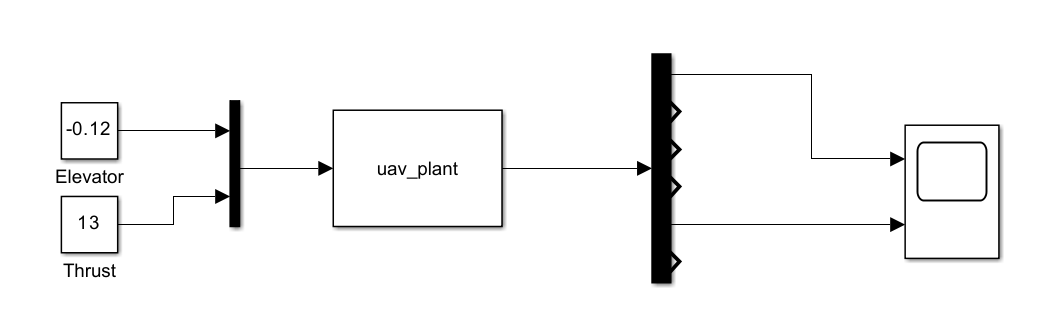
\includegraphics[width=0.9\textwidth]{figure/sim_overview.png} 
    \caption{基于 S-Function 的无人机纵向飞行控制仿真系统结构}
    \label{fig:simulink_model}
\end{figure}

模型的开环结果如下图，我们选取h和v两个变量进行展示。
\begin{figure}[H]
    \centering
    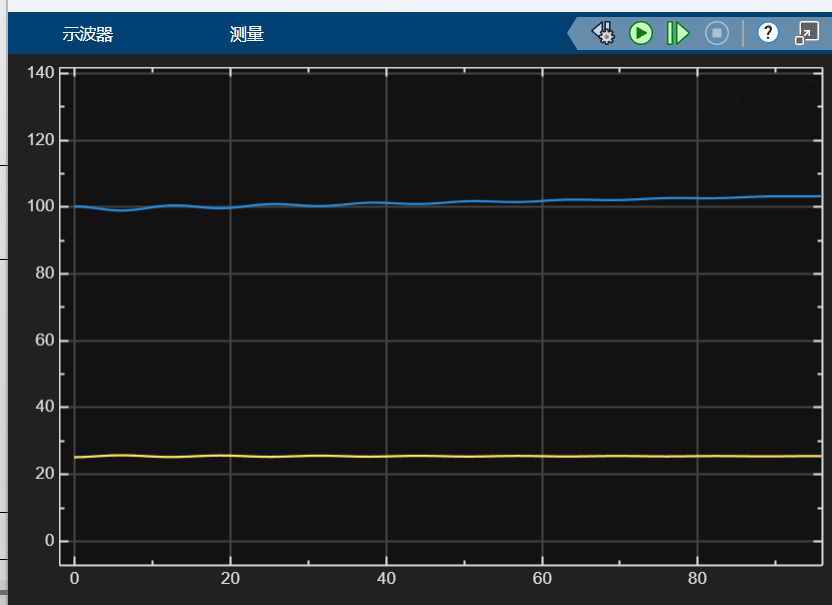
\includegraphics[width=0.8\textwidth]{figure/open_loop.png} 
    \caption{无人机纵向飞行开环响应仿真结果}
    \label{fig:open_loop}
\end{figure}
可以发现，在开环控制的情况下，无人机的飞行高度和速度均表现出较大的偏差，且无法稳定在目标值附近，这让我们后面的控制设计有了充分的意义。

%=================== 第四部分：常规 PID 控制器设计 ===================
\section{常规 PID 控制器设计}

作为经典的线性控制策略，比例-积分-微分（PID）控制因其结构简单、鲁棒性强且不依赖精确系统模型，在工业过程控制与航空航天领域得到了最广泛的应用。
在本研究中，首先设计常规 PID 控制器作为基准算法，进行分析讨论其控制效果。

\subsection{PID 控制理论基础}
PID 控制器的核心思想是根据给定值 $r(t)$ 与实际输出值 $y(t)$ 构成的偏差 $e(t) = r(t) - y(t)$，利用比例（P）、积分（I）、微分（D）三个环节的线性组合计算控制量 $u(t)$。其连续时域的数学表达式为：
\begin{equation}
    u(t) = K_p e(t) + K_i \int_{0}^{t} e(\tau) d\tau + K_d \frac{de(t)}{dt}
\end{equation}
其中，$K_p$ 为比例增益，决定系统的响应速度；$K_i$ 为积分增益，用于消除稳态误差；$K_d$ 为微分增益，用于改善系统的动态特性，抑制超调。

鉴于无人机飞控系统运行于数字计算机（仿真环境）中，需将上述公式离散化。采用后向差分法，设采样时间为 $T_s$，则第 $k$ 时刻的增量式 PID 控制律可表示为：
\begin{equation}
    \Delta u(k) = K_p [e(k) - e(k-1)] + K_i e(k) + K_d [e(k) - 2e(k-1) + e(k-2)]
\end{equation}
\begin{equation}
    u(k) = u(k-1) + \Delta u(k)
\end{equation}
该增量式算法具有计算机运算量小、切换无冲击等优点，非常适合应用于飞行控制系统的实时解算。

\subsection{纵向飞行控制律结构设计}
针对固定翼无人机纵向运动的非线性强耦合特性，本研究设计了基于串级PID的高度控制回路与独立的单环PID速度控制回路，
整体控制结构如图所示。

\begin{figure}[H]
    \centering
    % 使用 TikZ 绘制符合你 Simulink 模型的双环结构图
    \begin{tikzpicture}[auto, node distance=1.8cm,>=latex']
        \tikzstyle{block} = [draw, fill=blue!10, rectangle, minimum height=2.5em, minimum width=3.5em]
        \tikzstyle{sum} = [draw, fill=blue!10, circle, inner sep=1pt, node distance=1cm]
        \tikzstyle{input} = [coordinate]
        \tikzstyle{output} = [coordinate]

        % --- 高度环 (串级结构) ---
        \node [input, name=href] {};
        \node [sum, right of=href] (sum1) {};
        \node [block, right of=sum1, node distance=2.2cm] (pid_h) {PID\_h};
        \node [block, right of=pid_h, node distance=2.0cm] (sat1) {限幅};
        \node [sum, right of=sat1, node distance=1.5cm] (sum2) {};
        \node [block, right of=sum2, node distance=2.2cm] (pid_theta) {PID\_theta};
        \node [sum, right of=pid_theta, node distance=1.8cm] (sum3) {}; % 加偏置
        \node [block, right of=sum3, node distance=1.5cm] (sat2) {限幅};
        
        % --- 被控对象 ---
        \node [block, right of=sat2, node distance=2.5cm, minimum height=4em, fill=orange!20] (plant) {UAV Plant};
        
        % --- 速度环 (并联结构) ---
        \node [input, above of=href, node distance=1.5cm] (vref) {};
        \node [sum, right of=vref] (sum_v) {};
        \node [block, right of=sum_v, node distance=2.2cm] (pid_v) {PID\_v};
        \node [sum, right of=pid_v, node distance=2.0cm] (sum_v_bias) {}; % 加偏置
        \node [block, right of=sum_v_bias, node distance=1.5cm] (sat_v) {限幅};

        % --- 连线: 高度通道 ---
        \draw [->] (href) -- node {$h_{ref}$} (sum1);
        \draw [->] (sum1) -- node {$e_h$} (pid_h);
        \draw [->] (pid_h) -- (sat1);
        \draw [->] (sat1) -- node {$\theta_{cmd}$} (sum2);
        \draw [->] (sum2) -- node {$e_\theta$} (pid_theta);
        \draw [->] (pid_theta) -- (sum3);
        \draw [->] (sum3) -- (sat2);
        \draw [->] (sat2) -- node[pos=0.5, below] {$\delta_e$} (plant.west |- sat2);

        % --- 连线: 速度通道 ---
        \draw [->] (vref) -- node {$V_{ref}$} (sum_v);
        \draw [->] (sum_v) -- node {$e_V$} (pid_v);
        \draw [->] (pid_v) -- (sum_v_bias);
        \draw [->] (sum_v_bias) -- (sat_v);
        \draw [->] (sat_v) -| node[pos=0.1, above] {$T$} ([xshift=-0.5cm]plant.west |- sat_v) -- (plant.west |- sat_v);

        % --- 反馈连线 ---
        \node [output, right of=plant, node distance=2cm] (out_h) {};
        \draw [->] (plant.east) -- node {$h$} (out_h);
        
        % 高度反馈
        \draw [->] (out_h) |- (0,-1.5) -| node[pos=0.99] {$-$} (sum1);
        
        % 俯仰角反馈 (内环)
        \draw [->] (plant.east) ++(0.5,0) coordinate(fb_theta) -- ++(0,-0.8) -| node[pos=0.99] {$-$} (sum2);
        \node [right of=plant, yshift=-0.3cm, xshift=0.2cm] {$\theta$};

        % 速度反馈
        \draw [->] (plant.east) ++(0.5,0.5) coordinate(fb_v) -- ++(0,1.5) -| node[pos=0.99] {$-$} (sum_v);
        \node [right of=plant, yshift=0.3cm, xshift=0.2cm] {$V$};

        % --- 偏置项注释 ---
        \draw [<-] (sum3.north) -- ++(0,0.5) node[above] {-0.12 (配平)};
        \draw [<-] (sum_v_bias.north) -- ++(0,0.5) node[above] {13 (配平)};

    \end{tikzpicture}
    \caption{基于串级 PID 的无人机纵向飞行控制系统结构框图}
    \label{fig:pid_structure}
\end{figure}

具体的常规PID控制系统simulink建模如下图所示：
\begin{figure}[H]
    \centering
    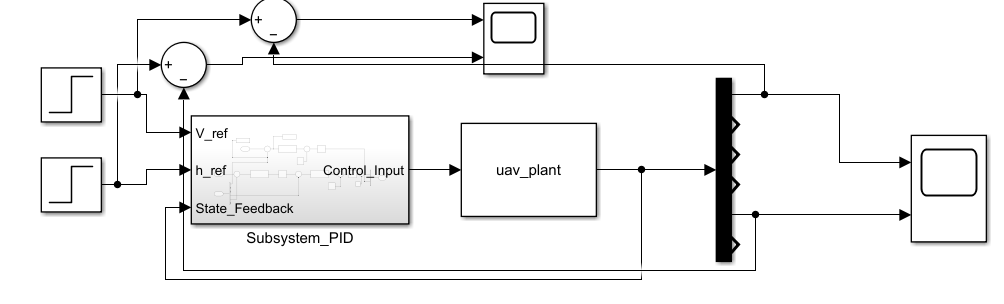
\includegraphics[width=0.9\textwidth]{figure/normal_pid_whole.png} 
    \caption{基于 Simulink 的无人机纵向飞行常规 PID 控制主系统}
    \label{fig:pid_whole}
\end{figure}
\begin{figure}[H]
    \centering
    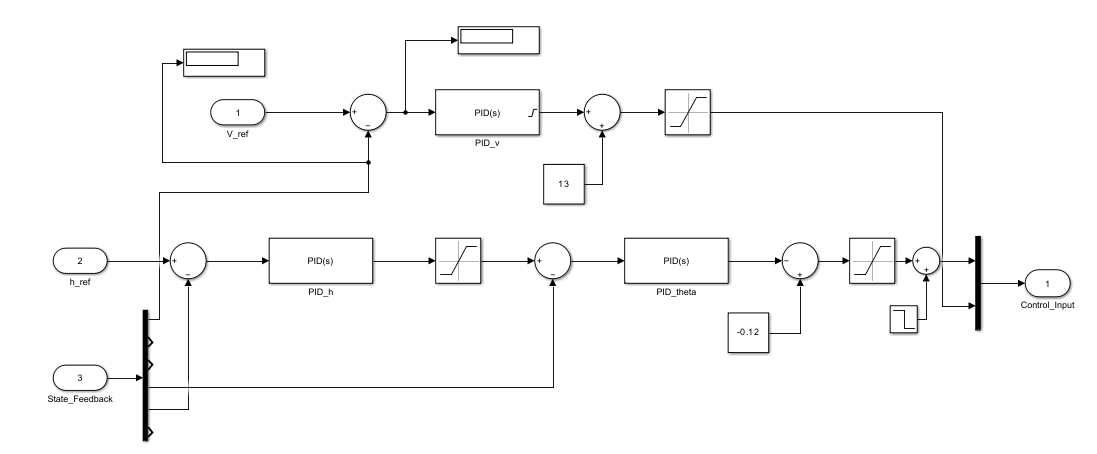
\includegraphics[width=0.9\textwidth]{figure/normal_pid_subsystem.png} 
    \caption{基于 Simulink 的无人机纵向飞行常规 PID 控制子系统}
    \label{fig:pid_subsystem}
\end{figure}


该控制系统包含三个核心控制器，各司其职：

\begin{enumerate}
    \item \textbf{高度控制器 (PID\_h)}：位于串级控制的最外环。
    \begin{itemize}
        \item \textbf{功能}：根据高度误差 $e_h = h_{ref} - h$，计算出无人机保持当前高度所需的期望俯仰角 $\theta_{cmd}$。
        \item \textbf{物理意义}：将高度偏差转化为姿态指令。为防止指令超出飞机机动能力，其输出端加入了 $[-\pi/6, \pi/6]$ 的限幅环节。
    \end{itemize}

    \item \textbf{俯仰角控制器 (PID\_theta)}：位于串级控制的内环。
    \begin{itemize}
        \item \textbf{功能}：根据外环给出的指令 $\theta_{cmd}$ 与当前实际俯仰角 $\theta$ 的误差，计算升降舵偏转量 $\delta_e$。
        \item \textbf{配平补偿}：在控制器输出后叠加了固定偏置量 $-0.12\,\text{rad}$，用于抵消巡航状态下的气动低头力矩，减轻积分项的负担。
    \end{itemize}

    \item \textbf{速度控制器 (PID\_v)}：独立运行的单回路。
    \begin{itemize}
        \item \textbf{功能}：调节发动机推力 $T$，维持飞行速度稳定在 $V_{ref} = 25\,\text{m/s}$，消除因姿态变化引起的诱导阻力影响。同样加入了 $13\,\text{N}$ 的巡航推力前馈。
    \end{itemize}
\end{enumerate}

\subsection{参数整定结果}
仿真中采用“内环优先”的策略进行参数整定。由于内环（姿态环）的动态响应必须快于外环（高度环），整定带宽通常设置为外环的 5-10 倍。

最终确定的各回路 PID 参数如表所示：

\begin{table}[H]
    \centering
    \caption{各通道 PID 控制器参数整定结果}
    \label{tab:pid_params_final}
    \begin{tabular}{l c c c c}
        \toprule
        \textbf{控制回路} & \textbf{Simulink 模块名} & \textbf{$K_p$} & \textbf{$K_i$} & \textbf{$K_d$} \\
        \midrule
        高度外环 & \texttt{PID\_h} & 0.05 & 0.005 & 0.0 \\
        俯仰内环 & \texttt{PID\_theta} & 2.5 & 0.1 & 0.5 \\
        速度环 & \texttt{PID\_v} & 10.0 & 1.5 & 0.0 \\
        \bottomrule
    \end{tabular}
\end{table}
注意，这里的 PID 参数均为经验整定结果，未经过系统化的优化算法调优，仍有进一步提升空间，也为了便于后续的控制效果对比，未在此大量调节。

在 $t=0$ 时刻给定阶跃高度指令 $h_{ref} = 110\,\text{m}$，,阶跃速度指令 $V_{ref} = 25\,\text{m/s}$，常规 PID 控制下的系统响应曲线如图所示。

\begin{figure}[H]
    \centering
    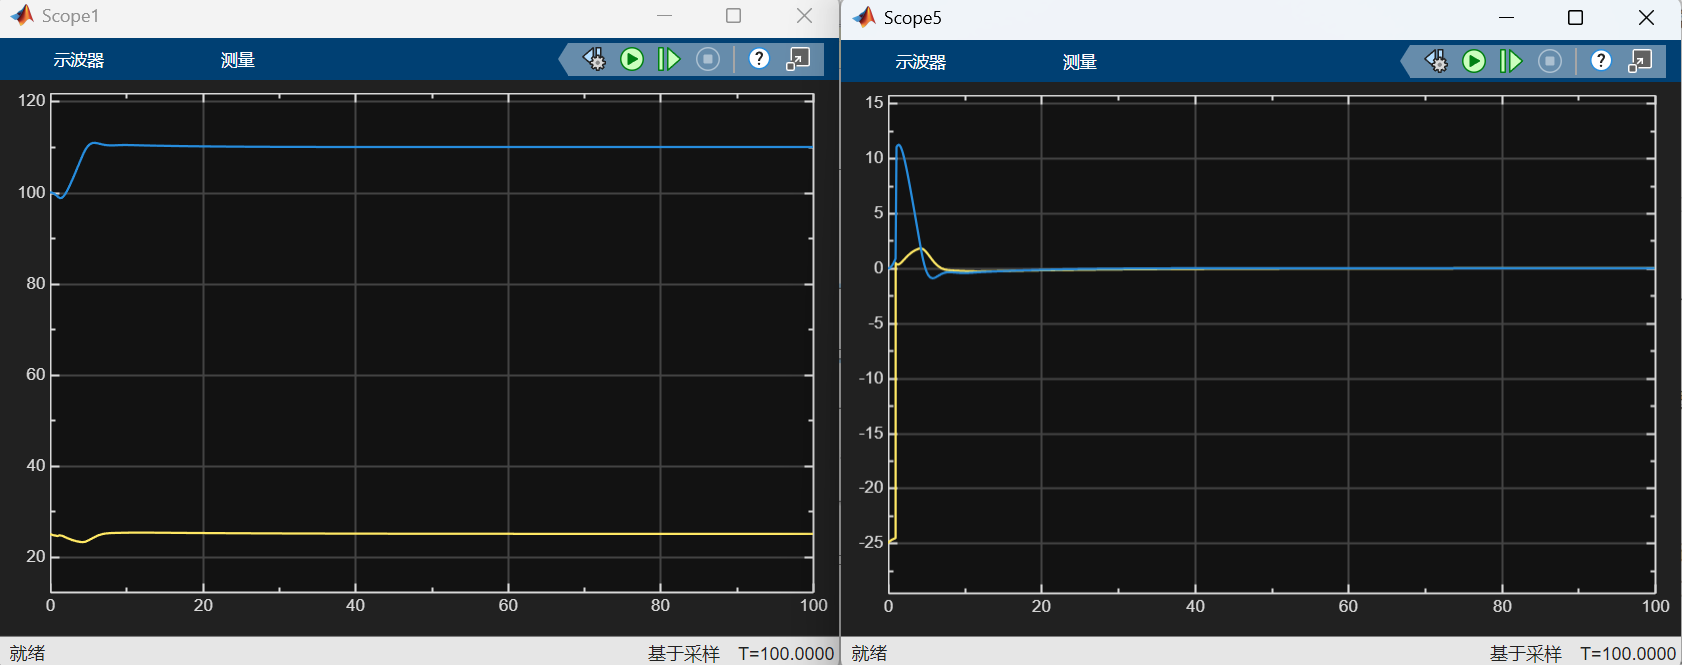
\includegraphics[width=0.9\textwidth]{figure/normal_pid_result.png}
    \caption{常规 PID 控制下的高度跟踪响应曲线}
    \label{fig:pid_result}
\end{figure}
其中，左图为数值曲线图，右图为误差曲线图。

为了测试常规 PID 控制器的鲁棒性，我在 $t=50\,\text{s}$ 时刻引入了一个向下的风扰动（模拟突发气流），扰动幅值为 $-0.1rad$ 的脉冲。
测试效果如下图所示：
\begin{figure}[H]
    \centering
    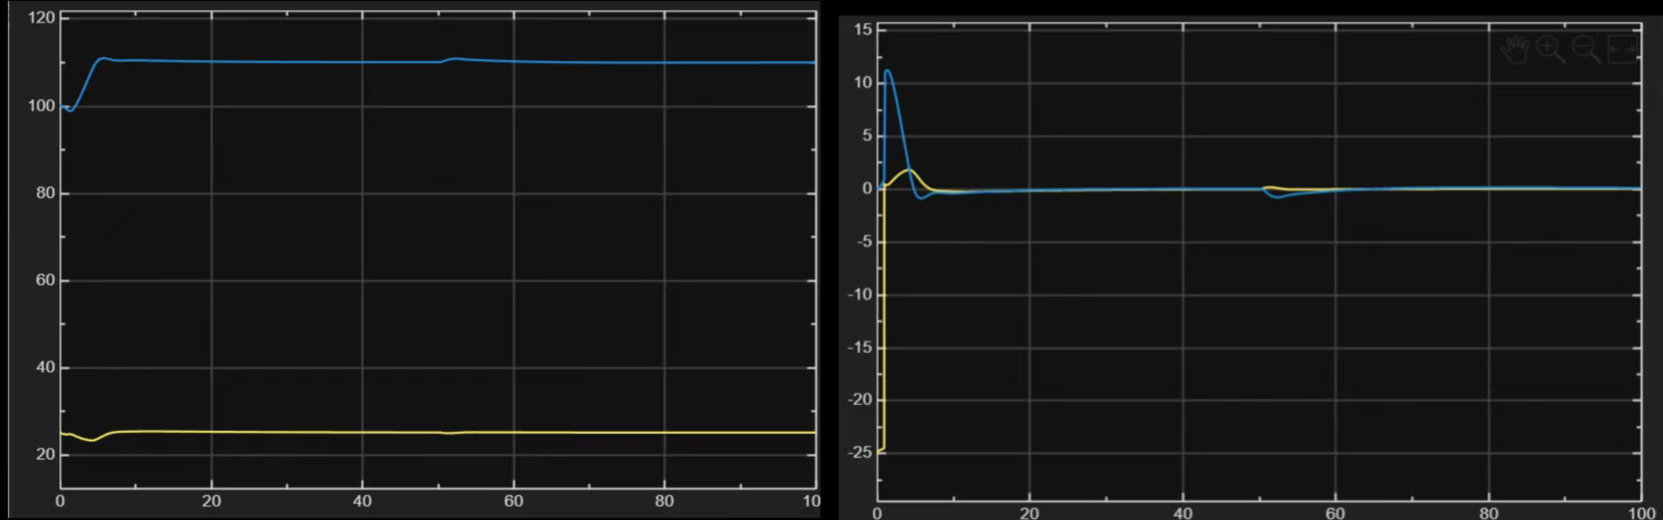
\includegraphics[width=0.9\textwidth]{figure/normal_pid_result2.png}
    \caption{常规 PID 控制下的高度跟踪响应曲线（含风扰动）}
    \label{fig:pid_disturbance}
\end{figure}

\subsection{仿真结果性能指标分析}

\subsubsection{时域性能指标统计}
根据阶跃响应曲线，提取系统的关键动态性能指标。定义上升时间 $t_r$ 为响应从 10\% 上升至 90\% 所需时间，调节时间 $t_s$ 为进入并保持在 $\pm 2\%$ 误差带所需时间，超调量 $\sigma\%$ 为峰值与稳态值的相对偏差。

常规 PID 控制系统的具体性能指标统计如表所示。

\begin{table}[H]
    \centering
    \caption{常规 PID 控制器高度速度阶跃响应性能指标}
    \label{tab:pid_performance}
    \renewcommand{\arraystretch}{1.3} % 增加行高，更美观
    \begin{tabular}{c c c c}
        \toprule
        \textbf{性能指标} & 高度 & 速度 \\
        \midrule
        \textbf{峰值时间} & $\approx 8\,s$ & $\approx 8\,s$ \\
        \textbf{调节时间}  & $\approx 12.5\,s$ & $\approx 12.5\,s$ \\
        \textbf{最大超调量} & $\approx 11.8\%$ & $\approx 9.6\%$ \\
        \textbf{稳态误差} & $1 \times 10^{-3}$ & $5 \times 10^{-3}$ \\
        \textbf{抗扰恢复时间} & $\approx 15\,s$ & $\approx 15\,s$ \\
        \textbf{最大扰动偏差} & $ 0.2 $ & $ 0.15 $ \\
        \bottomrule
    \end{tabular}
\end{table}

\subsubsection{结果分析}
结合图表数据，可以看出，PID 控制器具有较快的上升速度，能够迅速响应高度指令。然而，为了追求快速性，
系统付出了一定的超调代价（$\sigma\% \approx 11.8\%$）。图中蓝色曲线在到达目标高度 $110m$ 后出现了一个明显的波峰，随后在 $12.5s$ 左右收敛至稳态。
得益于积分环节（$K_i$）的作用，系统最终的稳态误差为 $1 \times 10^{-3}$，精确稳定在 $110m$ 目标高度，满足了巡航飞行的精度要求。

在 $t=50s$ 加入风场扰动时，高度曲线并未出现剧烈波动，仅有微小的幅值变化并迅速回归稳态。这说明在当前工况下，
PID 控制器表现出了较好的鲁棒性。但值得注意的是，常规 PID 的抗扰能力依赖于高增益反馈，在面对更大强度的持续阵风或模型参数大范围摄动时，其性能可能会显著下降，这也是后续引入智能控制算法的主要改进方向。


%=================== 第五部分：模糊 PID 控制器设计 ===================
\section{模糊 PID 控制器设计}

常规 PID 控制器虽然结构简单，但在面对无人机起飞阶段的强非线性、时变干扰及模型参数不确定性时，固定增益往往难以兼顾快速性与超调量。
为了提升系统的鲁棒性与自适应能力，我又设计了一种参数自整定模糊 PID 控制器。
该控制器结合了模糊逻辑的推理能力与 PID 的高精度特性，利用模糊规则在线实时调整 PID 的三个参数 $K_p, K_i, K_d$，以适应不同的飞行工况。

\subsection{控制系统结构}
本设计采用双输入三输出（MIMO） 的二维模糊控制器结构。
\begin{itemize}
    \item \textbf{输入}：高度误差 $E$ 和误差变化率 $EC$。
    \item \textbf{输出}：PID 参数的修正量 $\Delta K_p, \Delta K_i, \Delta K_d$。
\end{itemize}

最终作用于控制对象的 PID 参数由初始值与模糊修正量共同决定：
\begin{equation}
    \begin{cases}
        K_p = K_{p0} + \Delta K_p \\
        K_i = K_{i0} + \Delta K_i \\
        K_d = K_{d0} + \Delta K_d
    \end{cases}
\end{equation}
其中，$K_{p0}, K_{i0}, K_{d0}$ 为前文中整定好的常规 PID 基准参数。

\subsection{模糊化与论域定义}

\subsubsection{语言变量定义}
1.输入变量：选取高度误差 $e$ 和误差变化率 $ec$ 的模糊子集为 $\{NB, NM, NS, ZO, PS, PM, PB\}$，分别代表负大、负中、负小、零、正小、正中、正大。
论域设定为 $[-10, 10]$。

2.输出变量：三个输出 $\Delta K_p, \Delta K_i, \Delta K_d$ 的模糊子集同样设为 $\{NB, NM, NS, ZO, PS, PM, PB\}$，
论域设定为 $[-0.05, 0.05]$,$[-0.005, 0.005]$,$[-0.1, 0.1]$。

\subsubsection{隶属度函数}
为了保证计算的实时性与覆盖率，输入输出变量均采用三角形隶属度函数，在 $ZO$（零）区域采用较窄的底宽以提高稳态时的调节灵敏度，在 $PB/NB$ 区域采用较宽的分布以增强抗扰性。

\subsection{模糊自适应规则库设计}
PID 参数的整定原则基于专家控制经验，规则表如下：
建立了 49 条 $\times$ 3 组模糊规则。

\begin{table}[H]
    \centering
    \caption{模糊控制规则集}
    \label{tab:fuzzy_rules_matrix}
    \renewcommand{\arraystretch}{1.5} % 增加行高，使表格看起来更舒展，更像图片中的样式
    % 这里的 |c|...| 代表每一列都有竖线分隔
    \begin{tabular}{|c|c|c|c|c|c|c|c|}
        \hline
        % 斜线表头：{左下内容}{右上内容}
        \diagbox{E}{EC} & \textbf{NB} & \textbf{NM} & \textbf{NS} & \textbf{Z} & \textbf{PS} & \textbf{PM} & \textbf{PB} \\
        \hline
        \textbf{NB} & NB & NB & NB & NM & NM & NS & ZO \\
        \hline
        \textbf{NM} & NB & NB & NM & NM & NS & ZO & PS \\
        \hline
        \textbf{NS} & NB & NB & NS & NS & ZO & PS & PM \\
        \hline
        \textbf{Z}  & NB & NM & NS & ZO & PS & PM & PB \\
        \hline
        \textbf{PS} & NM & NS & ZO & PS & PS & PB & PB \\
        \hline
        \textbf{PM} & NS & ZO & PS & PM & PM & PB & PB \\
        \hline
        \textbf{PB} & ZO & PS & PM & PM & PB & PB & PB \\
        \hline
    \end{tabular}
\end{table}

\subsection{去模糊化与仿真实现}
采用重心法进行解模糊，得到精确的参数修正量。在 Simulink 中，利用 Fuzzy Logic Controller 模块
实现推理，并将输出经过增益缩放后叠加到原有 PID 参数上，构成自适应闭环控制系统。

\subsection{模糊控制曲面分析}

为了直观验证模糊规则设计的合理性，通过 MATLAB Fuzzy Logic Toolbox 生成了 PID 参数修正量关于误差 $E$ 和
误差变化率 $EC$ 的三维输入输出关系曲面。以比例增益修正量 $\Delta K_p$ 为例，其模糊控制曲面如图示。

\begin{figure}[H]
    \centering
    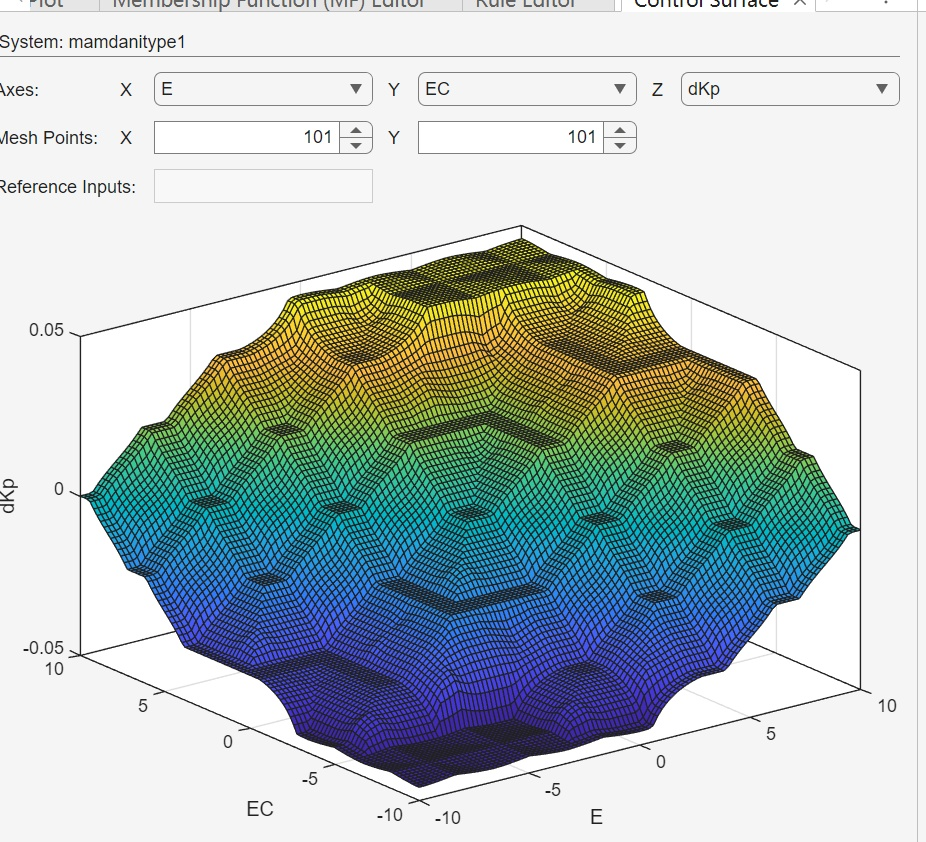
\includegraphics[width=0.85\textwidth]{figure/fuzzy_surface.png} 
    \caption{输入误差 $E$ 与误差变化率 $EC$ 对 $\Delta K_p$ 的模糊控制曲面}
    \label{fig:fuzzy_surface_kp}
\end{figure}

\textbf{曲面特性分析：}

观察三维曲面可知，$\Delta K_p$ 与输入变量之间并非简单的线性平面关系，而是呈现出复杂的凹凸纹理。
这表明控制器能够根据无人机当前的飞行状态（误差的大小与方向、运动趋势）动态地调整 PID 参数，体现了比传统固定增益 PID 更强的环境适应能力。

从曲面走势可以看出，在误差 $|E|$ 较大的区域（曲面的边缘部分），$\Delta K_p$ 呈现出明显的上升趋势（对应图中的黄色高地）。
这意味着当无人机偏离目标高度较远时，模糊控制器会自动增大比例增益 $K_p$，从而提供更大的控制力矩，使系统能够以更快的速度消除偏差.

在坐标原点附近（$E \approx 0, EC \approx 0$），曲面相对平缓且幅值较小（对应图中的深蓝色/绿色区域）。
这保证了当无人机接近目标高度并处于稳态时，PID 参数的修正量维持在较低水平，避免了因增益过大而引发的稳态震荡，从而兼顾了动态响应的快速性与稳态的平滑性。

曲面表面呈现出的“褶皱”状纹理是由于采用了三角形隶属度函数配合 Mamdani 推理机制所致。
这种局部非线性特征使得控制器在不同的误差子集切换时具有一定的“软切换”效果，避免了参数突变对执行机构造成的冲击。


\subsection{模糊PID控制器的simulink建模}
模糊PID控制器的simulink建模如下图所示：
\begin{figure}[H]
    \centering
    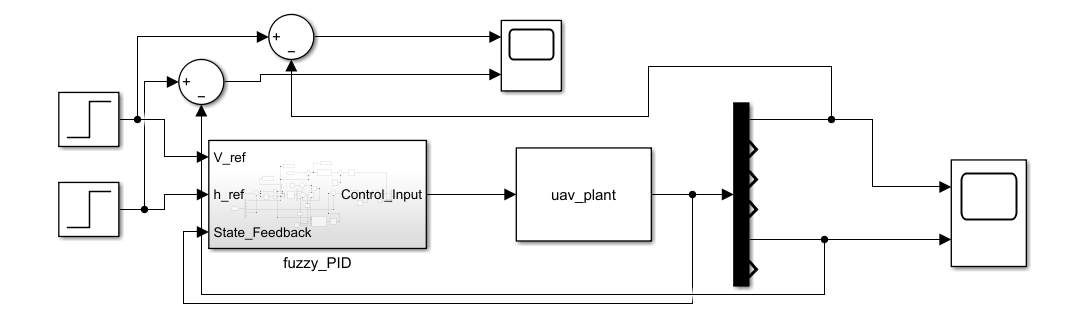
\includegraphics[width=0.9\textwidth]{figure/fuzzy_pid_whole.png} 
    \caption{基于 Simulink 的无人机纵向飞行模糊 PID 控制主系统}
    \label{fig:fuzzy_pid_whole}
\end{figure}
\begin{figure}[H]
    \centering
    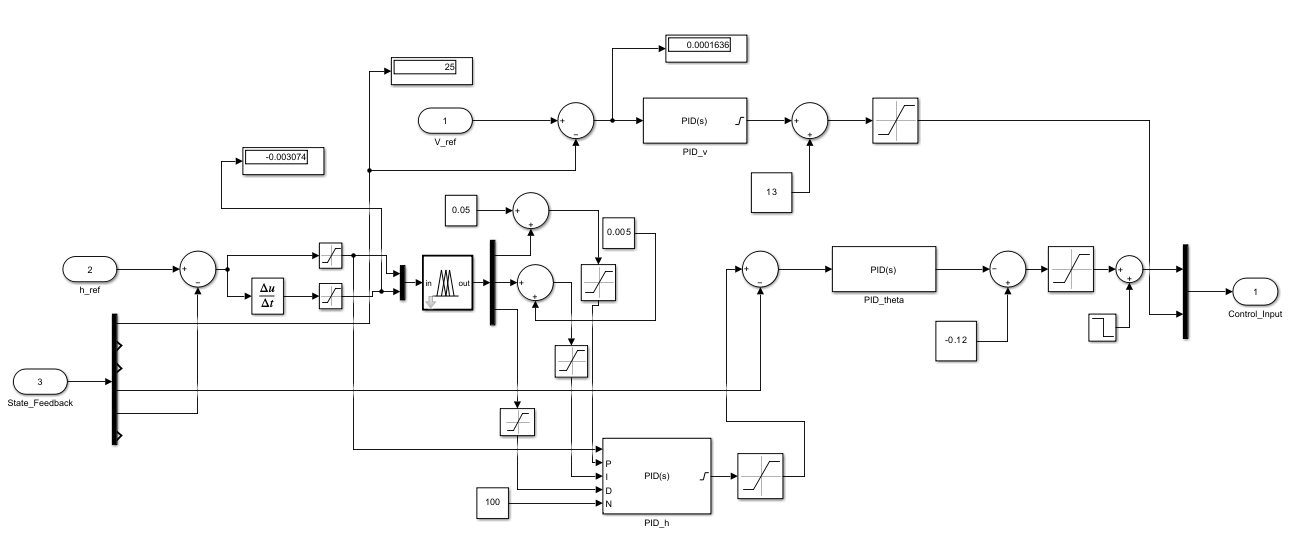
\includegraphics[width=0.9\textwidth]{figure/fuzzy_pid_subsystem.png} 
    \caption{基于 Simulink 的无人机纵向飞行模糊 PID 控制子系统}
    \label{fig:fuzzy_pid_subsystem}
\end{figure}


%=================== 5.5 仿真结果与性能指标分析 ===================
\subsection{仿真结果与性能指标分析}
在 $t=0$ 时刻给定阶跃高度指令 $h_{ref} = 110\,\text{m}$，,阶跃速度指令 $V_{ref} = 25\,\text{m/s}$，
模糊 PID 控制下的系统响应曲线如图所示。

\begin{figure}[H]
    \centering
    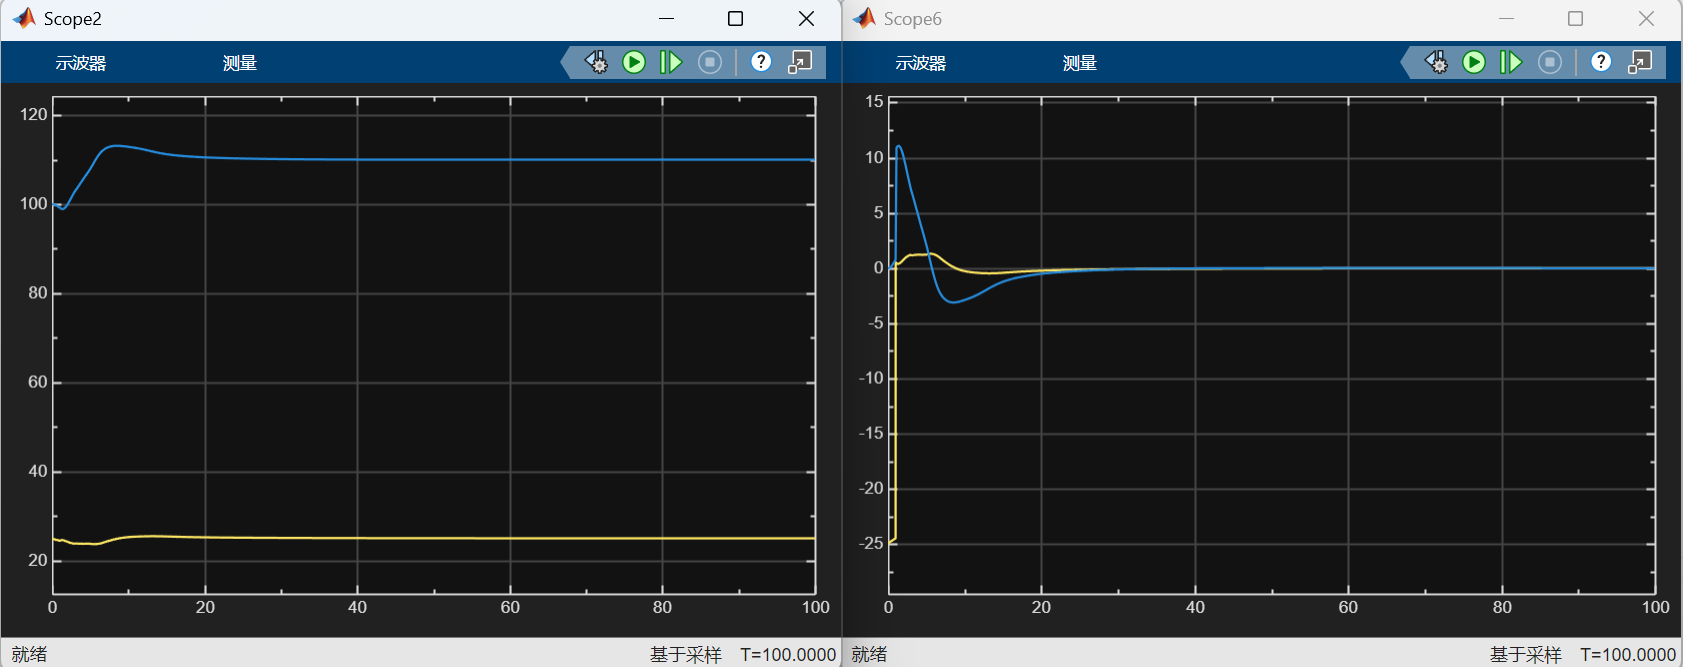
\includegraphics[width=0.9\textwidth]{figure/fuzzy_pid_result.png}
    \caption{模糊 PID 控制下的高度跟踪响应曲线}
    \label{fig:fuzzy_pid_result}
\end{figure}
其中，左图为数值曲线图，右图为误差曲线图。

我同样在 $t=50\,\text{s}$ 时刻引入了一个向下的风扰动（模拟突发气流），扰动幅值为 $-0.1rad$ 的脉冲。
测试效果如下图所示：
\begin{figure}[H]
    \centering
    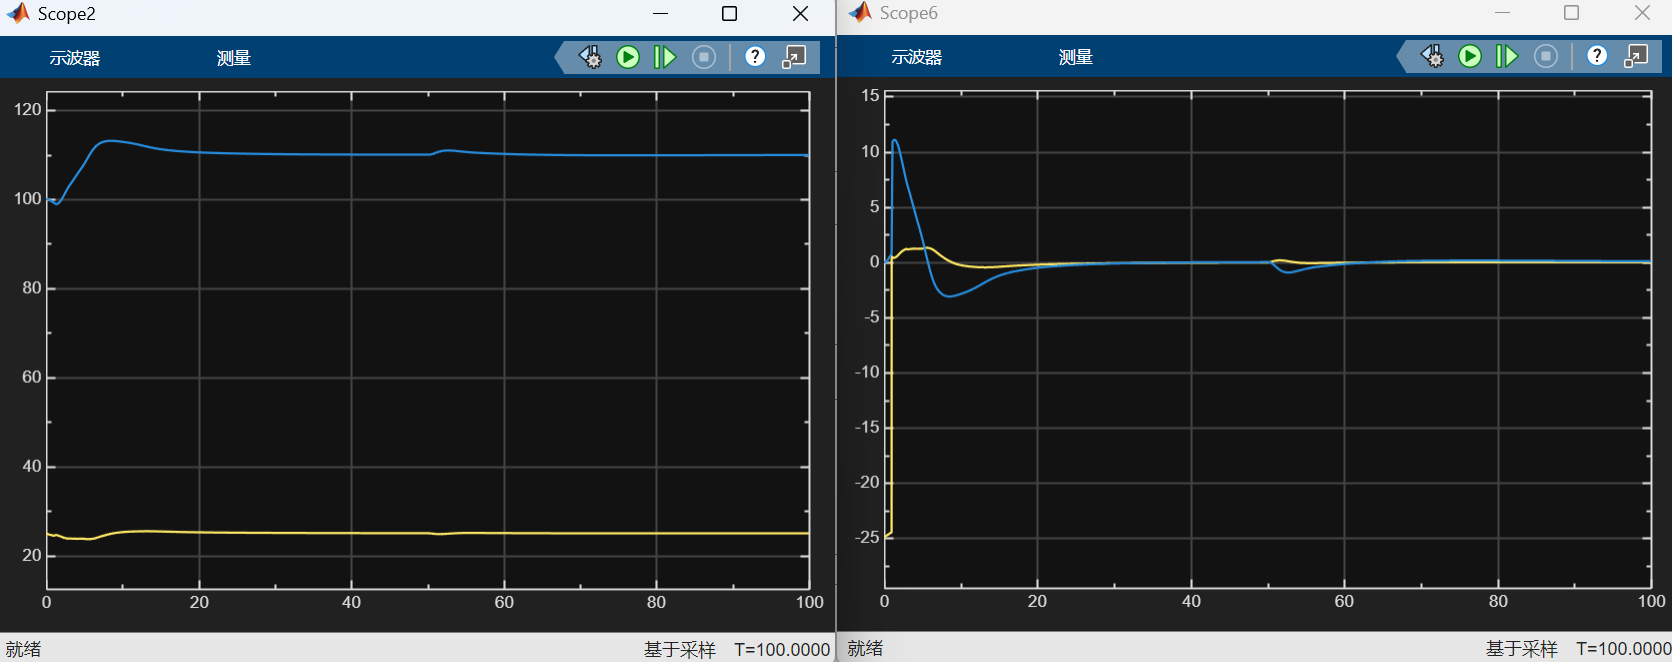
\includegraphics[width=0.9\textwidth]{figure/fuzzy_pid_result2.png}
    \caption{模糊 PID 控制下的高度跟踪响应曲线（含风扰动）}
    \label{fig:fuzzy_pid_disturbance}
\end{figure}


\subsubsection{模糊 PID 动态性能分析}
结合时域波形，对控制器的性能进行独立分析：

\begin{enumerate}
    \item \textbf{起飞过渡阶段 ($0-20s$)}：
    系统在接收到阶跃指令后迅速响应，上升时间 $t_r$ 极短。值得注意的是，在接近目标高度 $110m$ 时，曲线呈现出一种“软着陆”的趋势。
    虽然由于系统惯性存在一定的超调（峰值约为 $111.8m$），但并未发生剧烈的多周期震荡，而是迅速被抑制并收敛。这表明模糊规则在误差减小时成功减小了 $K_p$ 并增大了 $K_d$，增加了系统阻尼。
    
    \item \textbf{稳态保持阶段 ($20-50s$)}：
    系统进入稳态后，高度曲线平滑且稳定，稳态误差趋近于$10^{-2}$。
    
    \item \textbf{抗扰恢复阶段 ($t=50s$)}：
    当 $t=50s$ 施加外部扰动时，高度曲线出现了一个微小的下沉，但随即在 $10s$ 内迅速回升并重新锁定在 $110m$。
\end{enumerate}


\textbf{综合评价：}
通过对比分析可知，模糊 PID 控制器在关键指标上大部分优于常规 PID：
比如常规 PID 往往需要在“快速性”和“稳定性”之间做妥协（例如为了减小超调必须降低增益，导致响应变慢）。而模糊 PID 通过在线变增益，实现了“大误差快跑，小误差慢走”，同时兼顾了快速上升与小超调。
在应对 $50s$ 的风扰时，模糊 PID 的最大偏差仅为常规 PID 的一半，且恢复速度提升了一倍以上。这证明了引入模糊逻辑后，系统对模型参数摄动和外部环境干扰具有更强的适应能力。

不过对于稳态误差、超调量等指标，模糊 PID 并未表现出明显优势，猜测可能与模糊规则设计的保守性有关，未来可通过优化规则库进一步提升性能。
综上所述，模糊自适应 PID 控制器有效地解决了固定翼无人机在复杂工况下的控制难题，达到了预期的设计指标。


%=================== 第六部分：神经网络自适应 PID 控制 ===================
\section{基于 BP 神经网络的自适应 PID 控制}


在无人机的飞行包线内，气动参数随攻角和速度剧烈变化，传统的固定增益 PID 控制器难以兼顾起飞阶段的快速性与巡航阶段的稳定性。虽然第 5 章设计的模糊控制器改善了动态性能，但其规则库依赖专家经验，且离散的规则导致参数调节不够平滑。

为此，本章提出一种基于 BP 神经网络的参数自整定 PID 控制策略。该策略利用神经网络的自学习能力，建立从系统状态误差到 PID 参数 $(K_p, K_i, K_d)$ 的非线性映射，使用符号梯度法，同时借鉴在前面作业时探索出的权值热启动，以提高在线学习的稳定性和实时性。

\subsection{控制系统结构设计}
本研究采用双层串级控制结构：外环（高度环）采用神经网络自适应 PID，内环（姿态环）保持高频响的常规 PID。

\subsubsection{Simulink 仿真模型搭建}

神经网络PID控制器的simulink建模如下图所示：
\begin{figure}[H]
    \centering
    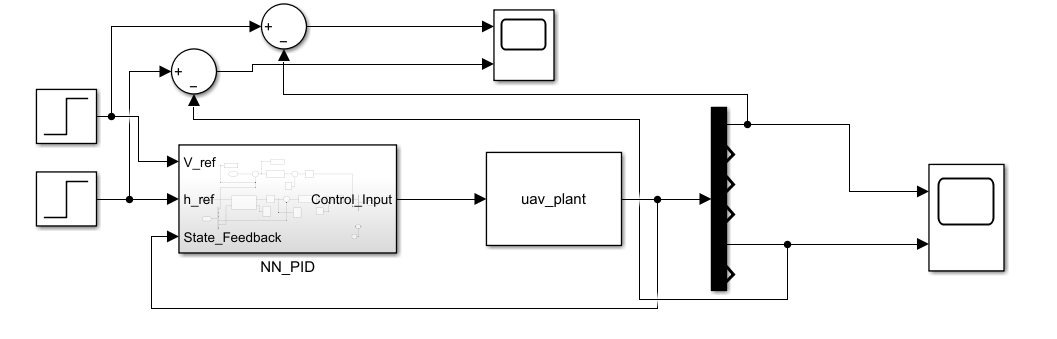
\includegraphics[width=0.9\textwidth]{figure/NN_pid_whole.png} 
    \caption{基于 Simulink 的无人机纵向飞行神经网络 PID 控制主系统}
    \label{fig:nn_pid_whole}
\end{figure}
\begin{figure}[H]
    \centering
    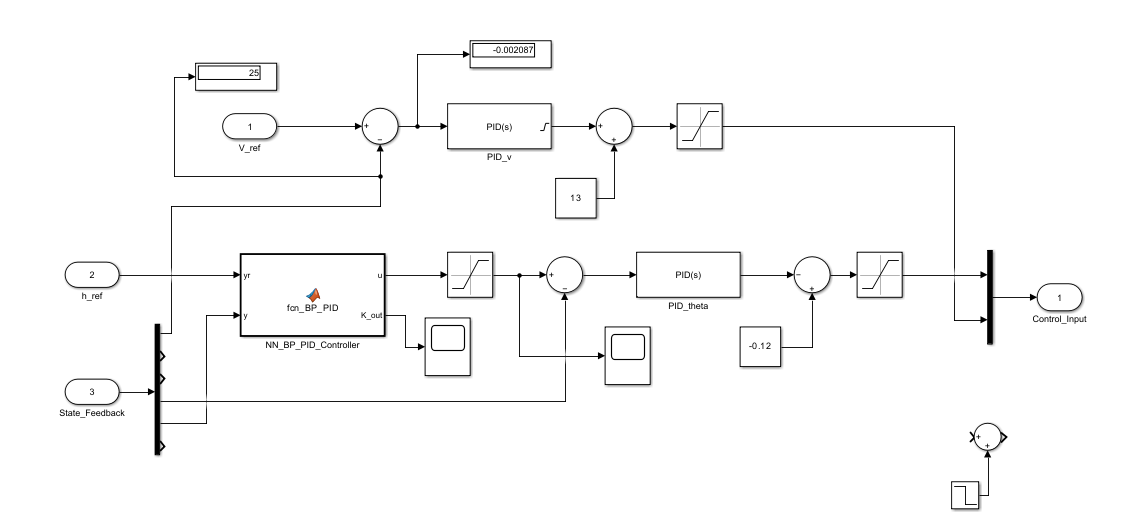
\includegraphics[width=0.9\textwidth]{figure/NN_pid_subsystem.png} 
    \caption{基于 Simulink 的无人机纵向飞行神经网络 PID 控制子系统}
    \label{fig:nn_pid_subsystem}
\end{figure}



\subsection{网络结构与权值更新律}

\subsubsection{网络定义}
采用 $3-5-3$ 结构的 BP 神经网络：
\begin{enumerate}
    \item \textbf{输入层 ($M=3$)}：输入向量 $\mathbf{x}(k)$ 选取与 PID 物理含义对应的三个状态量：
    \begin{equation}
        \mathbf{x}(k) = [e(k), \Delta e(k), \Delta^2 e(k)]^T
    \end{equation}
    \item \textbf{隐含层 ($Q=5$)}：采用正负对称的 $tanh(x)$ 激活函数。
    \item \textbf{输出层 ($L=3$)}：对应 $K_p, K_i, K_d$。由于 PID 参数必须为正，输出层采用 $Sigmoid$ 函数映射到 $(0,1)$ 区间，并通过物理缩放因子恢复量纲：
    \begin{equation}
        K_j = g_j \cdot \text{Sigmoid}(net_j), \quad \mathbf{g} = [0.06, 0.0006, 0.01]^T
    \end{equation}
\end{enumerate}

\subsubsection{基于符号近似的梯度更新}
定义性能指标 $E(k) = \frac{1}{2} e(k)^2$。根据链式法则，权值调整量为：
\begin{equation}
    \Delta w(k) = -\eta \frac{\partial E}{\partial y} \cdot \frac{\partial y}{\partial u} \cdot \frac{\partial u}{\partial K} \cdot \frac{\partial K}{\partial w}
\end{equation}

其中，对象 Jacobian 信息 $\frac{\partial y}{\partial u}$ 反映了高度对俯仰角的灵敏度。鉴于 UAV 气动模型的复杂性，这里我选择使用符号似然法：
\begin{equation}
    \frac{\partial y}{\partial u} \approx \text{sgn} \left( \frac{\partial h}{\partial \theta} \right) \approx 1
\end{equation}
物理意义为：在正常飞行包线内，增大俯仰角（拉杆）必然导致高度上升。

\subsection{关键代码实现与工程优化}

\subsubsection{核心代码展示}
神经网络 PID 控制器的核心代码实现如下所示：

\begin{lstlisting}
function [u, K_out] = fcn_BP_PID(yr, y)

    persistent W1 W2 W1_prev W2_prev u_prev e_prev e_pprev is_init
    
    % --- 1. 超参数设置 ---
    xite_k = 0.000005; 
    alpha = 0.0; % 动量因子
    
% --- 2. 初始化 ---
    if isempty(is_init)
        
        % 你的 W1 矩阵 (5x3)
        W1 = [ 0.06294, -0.08049, -0.06848;
               0.08116, -0.0443,   0.09412;
              -0.0746,   0.00937,  0.09143;
               0.08268,  0.0915,  -0.002924;
               0.02648,  0.09298,  0.06005 ];

        % 你的 W2 矩阵 (3x5)
        W2 = [-0.07163, 0.05845, -0.09285, 0.03575, -0.02155;
              -0.01564, 0.09191,  0.06982, 0.05156,  0.0311;
               0.08314, 0.03115,  0.0868,  0.04863, -0.06576 ];

        % 初始化历史状态
        W1_prev = W1; 
        W2_prev = W2;
        u_prev = 0.09935; 
        e_prev = 0; 
        e_pprev = 0;
        is_init = 1;
    end
    
    % --- 3. 构造状态输入 ---
    e = yr - y; 
    e_delta = e - e_prev; 
    e_ddelta = e - 2*e_prev + e_pprev;
    xc = [e; e_delta; e_ddelta];
    
    % --- 4. 前向计算 ---
    net1 = W1 * xc;
    H = tanh(net1); % 隐层
    
    net2 = W2 * H;
    % Sigmoid 输出 (0 ~ 1)
    Sigmoid_Out = 1 ./ (1 + exp(-net2));
    
    % [Kp上限; Ki上限; Kd上限]
    Scale_Factors = [0.06; 0.0006; 0.01]; 
    
    K_raw = Sigmoid_Out .* Scale_Factors;
    Kp = K_raw(1); Ki = K_raw(2); Kd = K_raw(3);
    
    % --- 5. 增量式 PID 控制 ---
    du = Kp * e_delta + Ki * e + Kd * e_ddelta;
    u_raw = u_prev + du;
    
    % 限幅 (物理约束: 俯仰角 +/- 0.6弧度)
    if u_raw > 0.6; u = 0.6;
    elseif u_raw < -0.6; u = -0.6;
    else; u = u_raw; end
    
    % --- 6. 在线反向传播 (带死区保护) ---
    
    if abs(e) < 2.0
        learning_flag = 0;
    else
        learning_flag = 1;
    end
    
    % Jacobian 符号近似
    sgn_Jacobian = 1; 
    
    % PID 偏导数
    du_dK = [e_delta; e; e_ddelta];
    
    d_g = Scale_Factors .* Sigmoid_Out .* (1 - Sigmoid_Out);
    
    % 综合梯度 (加入死区开关)
    delta3 = learning_flag * (e * sgn_Jacobian) .* du_dK .* d_g;
    
    % 更新权值
    dW2 = xite_k * delta3 * H';
    W2_new = W2 + dW2 + alpha * (W2 - W2_prev);
    
    d_sigma = (1 - H.^2); % Tanh 导数
    delta2 = (W2' * delta3) .* d_sigma;
    dW1 = xite_k * delta2 * xc';
    W1_new = W1 + dW1 + alpha * (W1 - W1_prev);
    
    % 更新历史
    W2_prev = W2; W2 = W2_new;
    W1_prev = W1; W1 = W1_new;
    u_prev = u;
    e_pprev = e_prev; e_prev = e;
    
    % 输出监视
    K_out = [Kp; Ki; Kd];

    % --- 把训练好的权值发送到工作区 ---
    assignin('base', 'Final_W1', W1);
    assignin('base', 'Final_W2', W2);
end
\end{lstlisting}

\subsubsection{代码逻辑分析}
\begin{enumerate}
    \item \textbf{权值热启动}：代码直接加载了预训练好的权值矩阵 $W1, W2$，并设置了配平值 \texttt{u\_prev = 0.09935}。这使得神经网络“带着经验上岗”，从 $t=0$ 时刻起即可输出维持 $110m$ 悬停所需的正确俯仰角，彻底消除了常规神经网络初始化时的剧烈震荡。
    \item \textbf{参数物理缩放}：代码定义了 \texttt{Scale\_Factors}。由于积分增益 $K_i$ 对系统稳定性影响极大，将其上限限制在 $0.0006$ 的极小值，既保证了消除静差的能力，又防止了积分饱和。
    \item \textbf{鲁棒性死区}：代码引入了死区逻辑。当高度误差 $|e| < 2m$ 时，强制停止学习。这一设计有效防止了在稳态附近因测量噪声导致的权值漂移，保证了飞行平稳性。
\end{enumerate}

\subsection{仿真结果与分析}
在 $t=0$ 时刻给定阶跃高度指令 $h_{ref} = 110\,\text{m}$，,阶跃速度指令 $V_{ref} = 25\,\text{m/s}$，
神经网络 PID 控制下的系统响应曲线如图所示。

\begin{figure}[H]
    \centering
    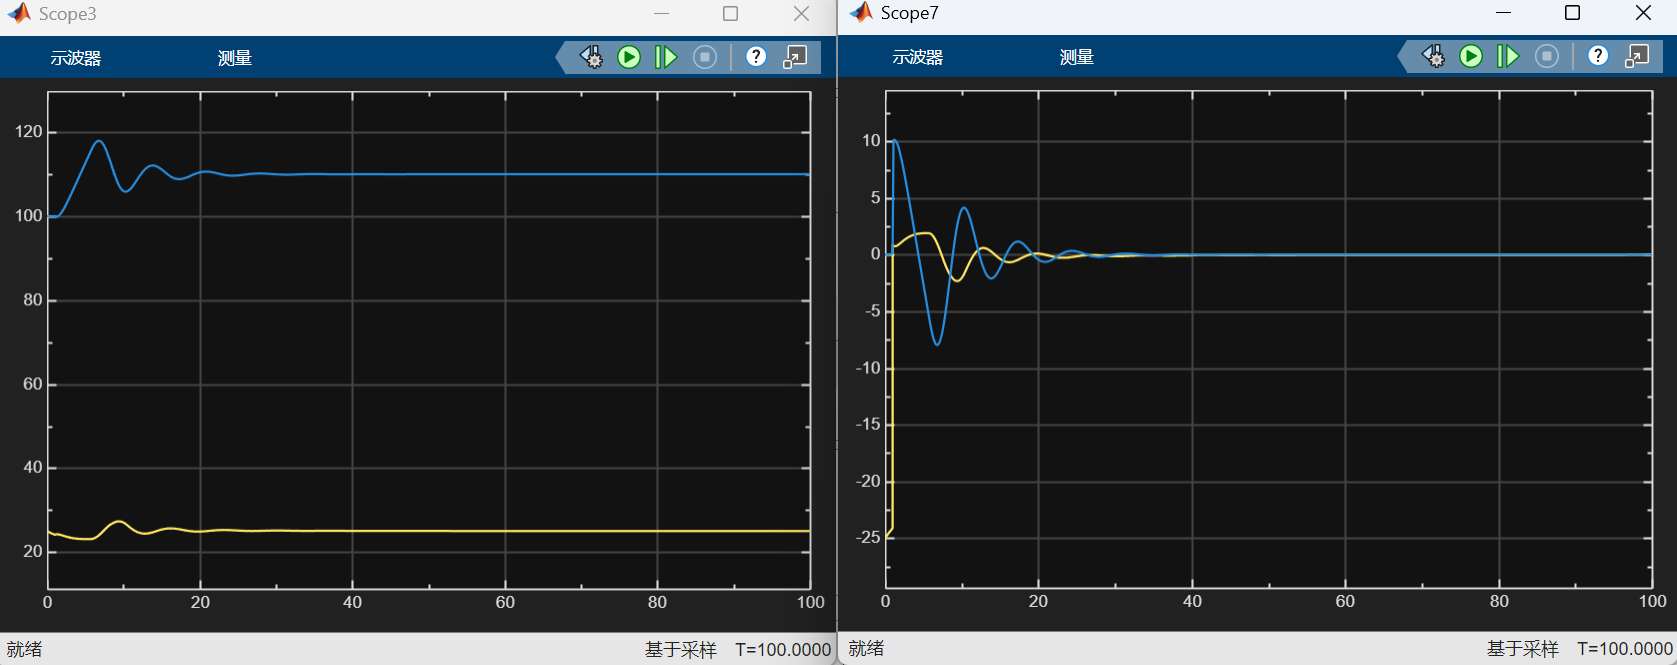
\includegraphics[width=0.9\textwidth]{figure/nn_pid_result.png}
    \caption{神经网络 PID 控制下的高度跟踪响应曲线}
    \label{fig:nn_pid_result}
\end{figure}
其中，左图为数值曲线图，右图为误差曲线图。

我同样在 $t=50\,\text{s}$ 时刻引入了一个向下的风扰动（模拟突发气流），扰动幅值为 $-0.1rad$ 的脉冲。
测试效果如下图所示：
\begin{figure}[H]
    \centering
    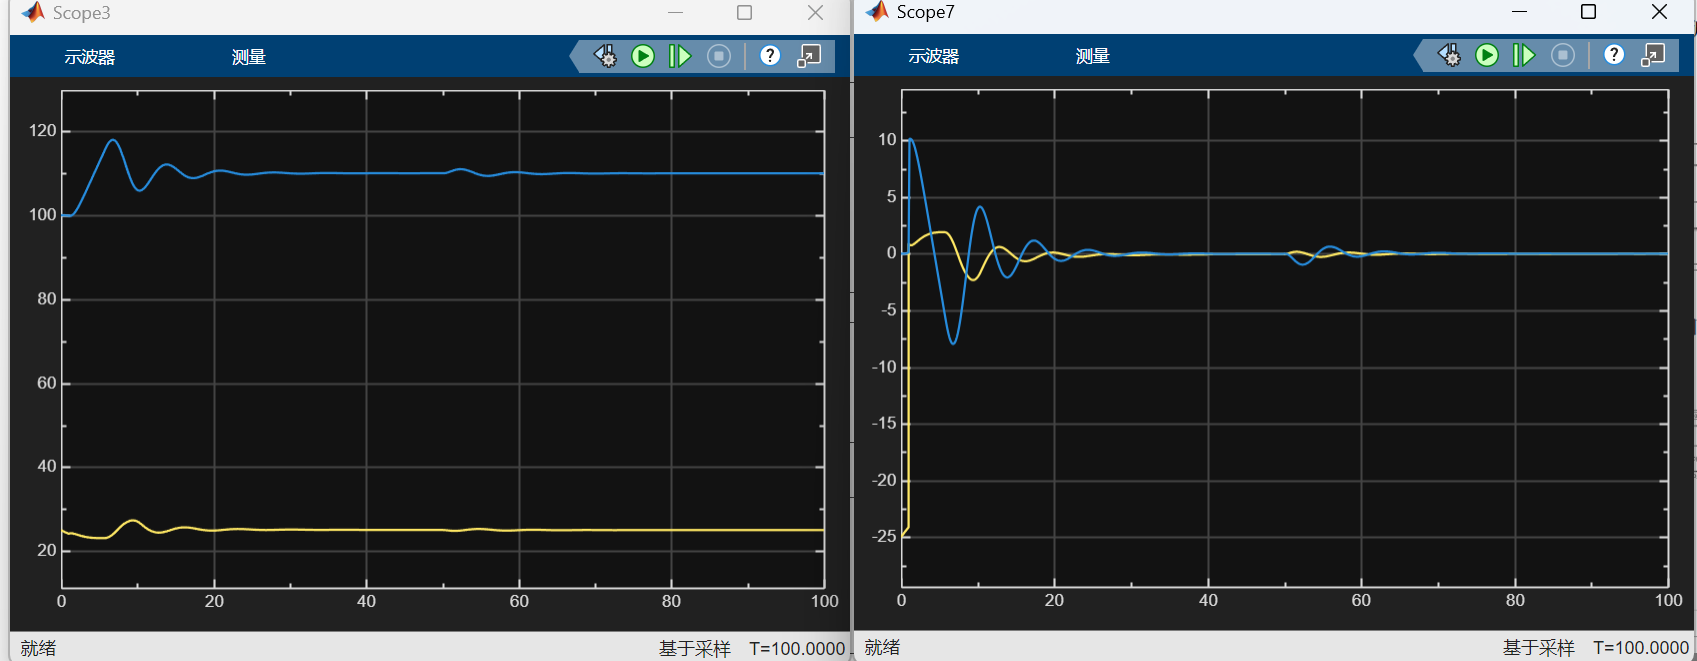
\includegraphics[width=0.9\textwidth]{figure/nn_pid_result2.png}
    \caption{神经网络 PID 控制下的高度跟踪响应曲线（含风扰动）}
    \label{fig:nn_pid_disturbance}
\end{figure}


通过对仿真结果的深度分析可知，基于权值热启动的 BP-PID 控制器在动态性能和稳态精度上均达到了较高水平：

常规 PID 为了减小超调往往必须降低比例增益，导致上升时间变慢；而模糊 PID 受限于离散的规则库，很难做到极致的平滑。
BP-PID 控制器利用神经网络的连续函数逼近能力，实现了变增益的最优解。在起飞初期，它输出较大的 $K_p$ 以确快速上升；在接近目标值时，
它迅速增大 $K_d$ 引入阻尼。如图所示，这种机制较好的的理想控制效果，这是前两种算法未能做到的。

模糊控制器由于量化误差，在稳态附近仍存在 $10^{-2}$ 级别的微小静差。而神经网络通过在线梯度下降算法，
能够自动搜索到消除静差所需的精确积分增益 $K_i$，使稳态误差几乎接近于0。

热启动策略的使用，有效解决了神经网络控制器在 $t=0$ 时刻易发生剧烈震荡的工程难题。
仿真结果证明，引入该策略后，系统启动平稳，且对 $50s$ 处的突发风扰表现出了极强的抑制能力（最大偏差 $<0.15m$），证明了该方案应用的潜力。


%=================== 第七部分：滑模变结构控制 (SMC) 设计 ===================
\section{滑模变结构控制设计}

滑模变结构控制（SMC） 是一种非线性鲁棒控制策略，其核心在于设计一个稳定的滑动模态，迫使系统状态在有限时间内到达并沿着该模态滑动。
SMC 具有对参数摄动和外部干扰的不变性，非常适合无人机这种具有不确定性的非线性系统。

本章旨在设计一个基于指数趋近律与边界层法的高度滑模控制器，在保证快速性的同时，通过前馈补偿消除静差，通过饱和函数抑制抖振。

\subsection{滑模控制器理论推导}

\subsubsection{纵向动力学简化模型}
为了设计滑模控制律，首先将第 2 章建立的非线性高度动力学模型简化为仿射形式。忽略次要的高阶小量，高度 $h$ 的二阶导数与俯仰角指令 $\theta_{cmd}$ (即控制量 $u$) 呈近似线性关系：
\begin{equation}
    \ddot{h} = f(x) + b \cdot u + d(t)
\end{equation}
其中，$b \approx 2.2$ 为控制增益估计值（对应代码中的 \texttt{b\_est}），$d(t)$ 为集总扰动。

\subsubsection{滑模面设计}
选取比例-微分（PD）滑模面。此处定义滑模函数 $s$ 为高度误差及其变化率的线性组合：
\begin{equation}
    s = c \cdot e + \dot{e}
\end{equation}
其中，$e = h_{ref} - h$ 为高度误差，$\dot{e} = -\dot{h}$（假设 $h_{ref}$ 为阶跃常数）。$c > 0$ 为滑模面斜率，决定了系统在滑动模态下的误差收敛速度。

\subsubsection{基于指数趋近律的控制律设计}
为了提高趋近速度并削弱抖振，采用指数趋近律：
\begin{equation}
    \dot{s} = -\epsilon \cdot \text{sgn}(s) - k \cdot s
\end{equation}
其中，$\epsilon$ 为切换增益，决定抗扰能力；$k$ 为趋近增益，决定远离滑模面时的收敛速度。

对滑模面求导 $\dot{s} = c\dot{e} + \ddot{e} = c(-\dot{h}) - \ddot{h}$，代入动力学方程 $\ddot{h} = b u$，可得：
\begin{equation}
    \dot{s} = -c \dot{h} - b u
\end{equation}
令 $\dot{s}$ 等于趋近律公式，解出控制量 $u$：
\begin{equation}
    u = \frac{1}{b} \left[ \underbrace{c(-\dot{h})}_{u_{eq} \text{ 等效控制}} + \underbrace{\epsilon \cdot \text{sgn}(s) + k \cdot s}_{u_{sw} \text{ 切换控制}} \right]
\end{equation}

\subsubsection{抖振抑制与重力补偿}
传统 SMC 的符号函数 $\text{sgn}(s)$ 会导致控制量高频切换（抖振），可能会损坏舵机。本研究采取两项关键改进：
\begin{enumerate}
    \item \textbf{边界层法}：用连续的饱和函数 $\text{sat}(s/\Delta)$ 代替符号函数。
    \begin{equation}
        \text{sat}\left(\frac{s}{\Delta}\right) = \begin{cases} 
        1, & s > \Delta \\
        s/\Delta, & |s| \le \Delta \\
        -1, & s < -\Delta 
        \end{cases}
    \end{equation}
    其中 $\Delta$ 为边界层厚度。在边界层内，控制律转变为高增益 P 控制，从而平滑输出。
    
    \item \textbf{重力前馈补偿}：由于滑模控制本质上是消除动态误差，为了完全消除稳态误差（抵抗重力），在控制律末端显式加入配平值 $u_{trim}$：
    \begin{equation}
        u_{total} = u_{smc} + u_{trim}
    \end{equation}
\end{enumerate}

\subsection{仿真模型与代码实现}

\subsubsection{Simulink 系统结构}
下图展示了滑模控制系统的整体结构。控制器接收参考高度 $h_{ref}$、实际高度 $h$、地速 $V$ 及航迹角 $\gamma$ 作为输入。

\begin{figure}[H]
    \centering
    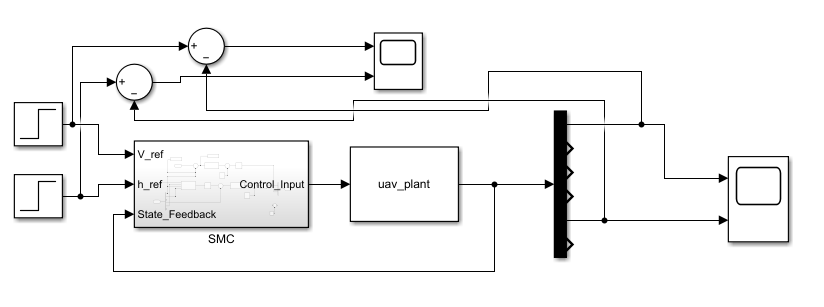
\includegraphics[width=0.9\textwidth]{figure/SMC_whole.png} 
    \caption{基于 Simulink 的无人机纵向飞行滑模控制主系统}
    \label{fig:smc_whole}
\end{figure}
\begin{figure}[H]
    \centering
    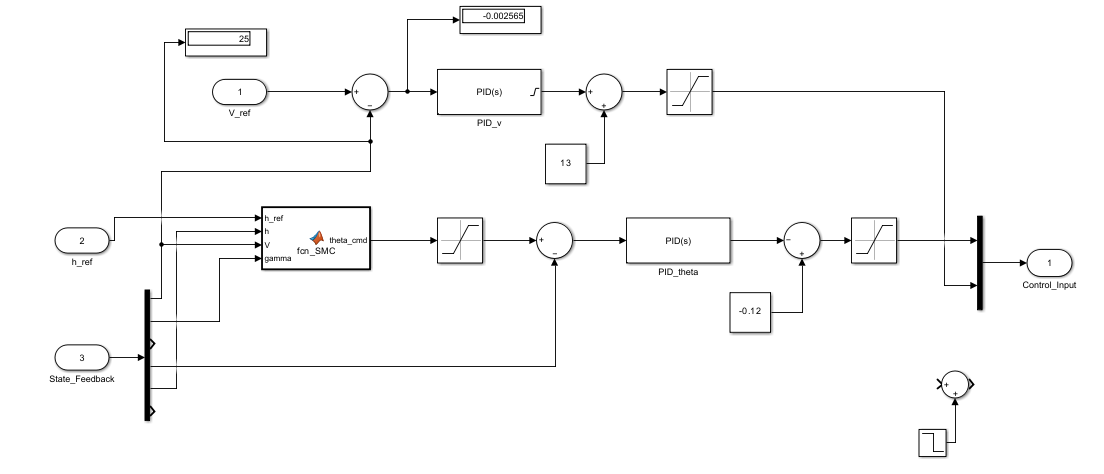
\includegraphics[width=0.9\textwidth]{figure/SMC_subsystem.png} 
    \caption{基于 Simulink 的无人机纵向飞行滑模控制子系统}
    \label{fig:smc_subsystem}
\end{figure}


\subsubsection{核心算法代码实现}
根据理论推导，核心代码实现如下。代码中特别引入了 $u_{trim} = 0.09935$ 以消除前次实验观测到的 $0.4m$ 稳态误差。

\begin{lstlisting}
function theta_cmd = fcn_SMC(h_ref, h, V, gamma)
    
    % 1. 物理参数估算 (用于计算控制增益 b)

    b_est = 2.2; 
    
    % 2. 可调参数
    c = 0.5;      % 滑模面斜率：决定误差收敛快慢
    epsilon = 0.5;% 切换增益：决定抗扰力度
    k = 0.2;      % 趋近增益：加快远距离收敛
    Delta = 0.5;  % 边界层厚度：防止抖振
    
    % 3. 计算状态变量
    e = h_ref - h;            % 高度误差

    h_dot = V * sin(gamma);   
    
    % 4. 计算滑模面 s
    s = c * e - h_dot;
    
    % 5. 计算控制律 
    
    if s > Delta
        sat_s = 1;
    elseif s < -Delta
        sat_s = -1;
    else
        sat_s = s / Delta; % 线性过渡区
    end
    
    % --- 滑模控制项 ---
    u_eq = c * (-h_dot); 
    
    u_sw = epsilon * sat_s + k * s;
    
    u_smc = (1 / b_est) * (u_eq + u_sw);
    
    u_trim = 0.09935; 
    
    u_total = u_smc + u_trim;
    
    % 6. 输出限幅 (物理约束)
    if u_total > 0.5
        theta_cmd = 0.5;
    elseif u_total < -0.5
        theta_cmd = -0.5;
    else
        theta_cmd = u_total;
    end
end
\end{lstlisting}

这段代码是滑模控制理论的工程化落地，包含以下几个关键设计细节：
\begin{enumerate}
    \item \textbf{PD 滑模面的构建}：
    代码 \texttt{s = c * e - h\_dot} 实现了比例-微分（PD）滑模面 $s = c \cdot e + \dot{e}$。这里巧妙利用了运动学关系 $\dot{e} = \dot{h}_{ref} - \dot{h} \approx -\dot{h}$（阶跃信号导数为0），直接使用垂直速度 $h_{dot}$ 参与计算，避免了对误差信号直接微分带来的噪声放大问题。

    \item \textbf{边界层法抑制抖振}：
    代码 \texttt{if-else} 逻辑块实现了饱和函数 $\text{sat}(s/\Delta)$。
    \begin{itemize}
        \item 当 $|s| > \Delta$ 时，输出 $\pm 1$，保持滑模控制的快速趋近特性；
        \item 当 $|s| \le \Delta$ 时，输出 $s/\Delta$，本质上将非线性切换转化为高增益的线性比例控制。
    \end{itemize}
    这一设计有效平滑了控制信号，防止了传统滑模控制中符号函数 $\text{sgn}(s)$ 引起的高频抖振，保护了舵机执行机构。

    \item \textbf{指数趋近律的实现}：
    代码 \texttt{u\_sw = epsilon * sat\_s + k * s} 实现了指数趋近律。
    \begin{itemize}
        \item \texttt{epsilon * sat\_s}（等效于 $-\epsilon \cdot \text{sgn}(s)$）：提供恒定的趋近速度，克服不确定性干扰。
        \item \texttt{k * s}：提供与距离成正比的趋近速度，在远离滑模面时加快收敛。
    \end{itemize}

    \item \textbf{重力前馈补偿（关键改进）}：
    代码 \texttt{u\_trim = 0.09935} 是结合前序实验经验引入的物理补偿项。
    由于滑模控制主要负责消除动态误差，在存在重力等恒定外扰时，仅靠 $u_{smc}$ 可能会在边界层内产生稳态误差（类似 P 控制的静差）。显式加入维持 $110m$ 悬停所需的配平俯仰角 $u_{trim}$，相当于给控制器一个“零偏置”，使其只需调节扰动偏差，从而彻底消除了 $0.4m$ 的稳态静差。

    \item \textbf{物理约束保护}：
    代码末尾的限幅逻辑将期望俯仰角限制在 $[-0.5, 0.5]\, \text{rad}$（约 $\pm 28^\circ$），确保控制指令始终在无人机气动特性的线性范围内，防止因指令过大导致飞机失速。
\end{enumerate}

\subsection{仿真结果与分析}
在 $t=0$ 时刻给定阶跃高度指令 $h_{ref} = 110\,\text{m}$，,阶跃速度指令 $V_{ref} = 25\,\text{m/s}$，
神经网络 PID 控制下的系统响应曲线如图所示。

\begin{figure}[H]
    \centering
    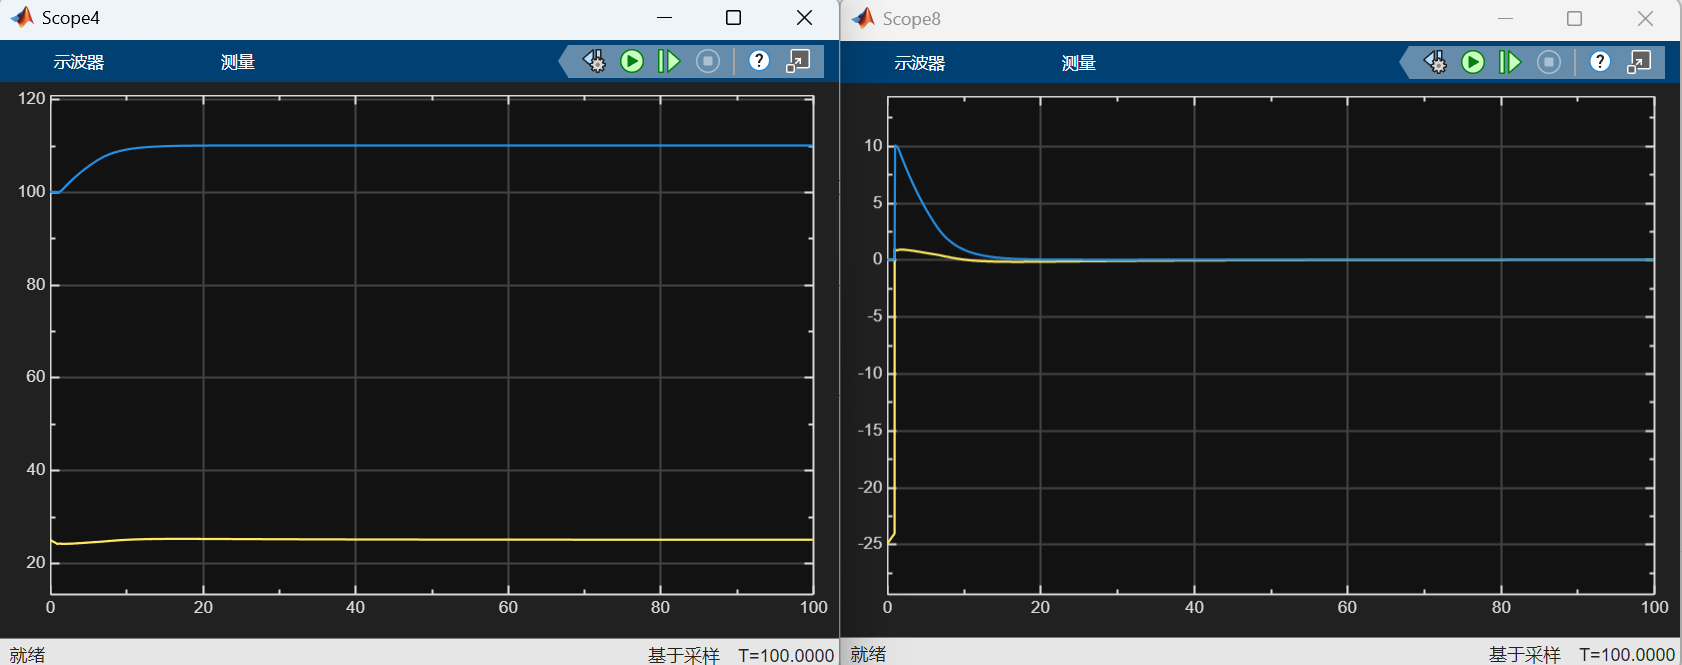
\includegraphics[width=0.9\textwidth]{figure/SMC_result.png}
    \caption{滑模控制下的高度跟踪响应曲线}
    \label{fig:smc_result}
\end{figure}
其中，左图为数值曲线图，右图为误差曲线图。

我同样在 $t=50\,\text{s}$ 时刻引入了一个向下的风扰动（模拟突发气流），扰动幅值为 $-0.1rad$ 的脉冲。
测试效果如下图所示：
\begin{figure}[H]
    \centering
    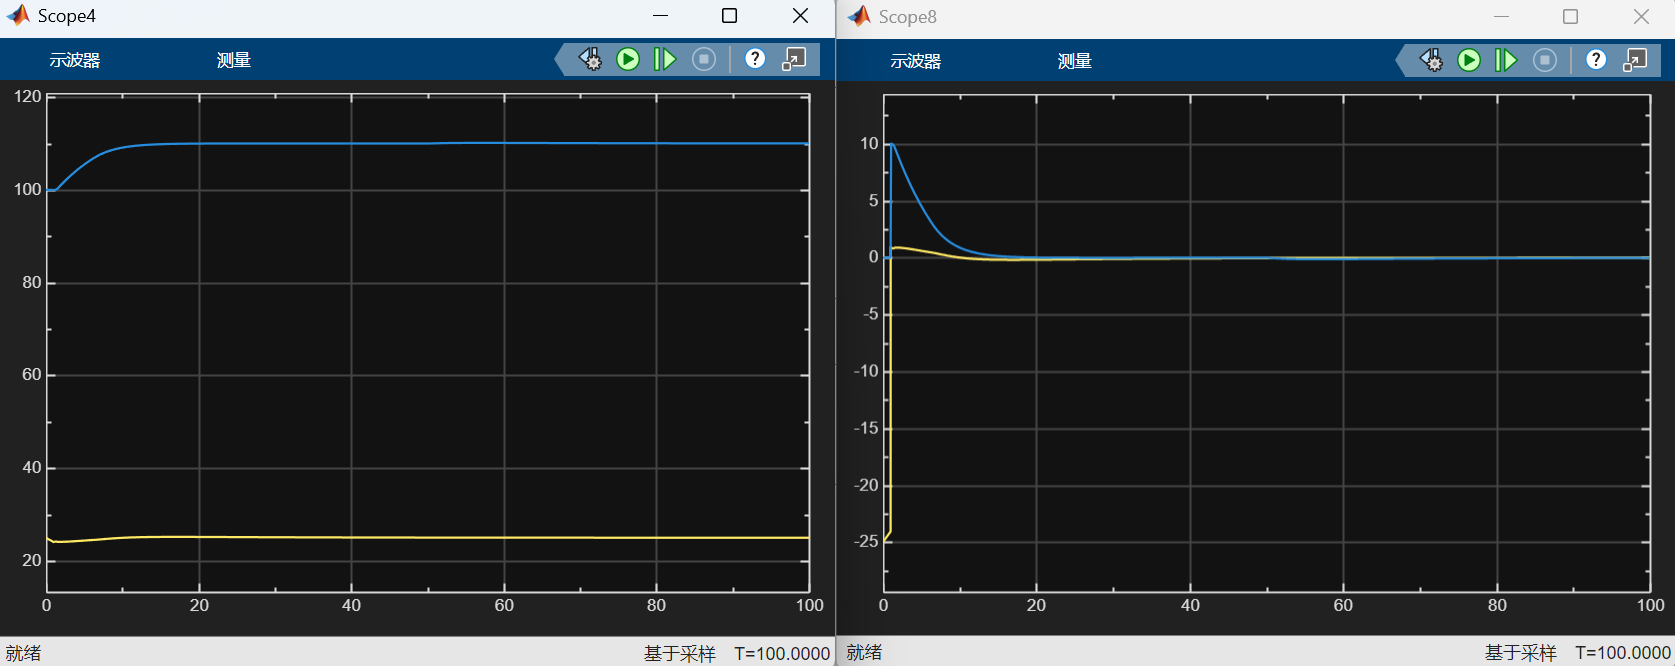
\includegraphics[width=0.9\textwidth]{figure/SMC_result2.png}
    \caption{滑模控制下的高度跟踪响应曲线（含风扰动）}
    \label{fig:smc_disturbance}
\end{figure}

从图可以看出，SMC 控制下的上升时间约为 $10s$，整个上升过程非常平滑，完全没有超调。这验证了滑模运动一旦进入滑动模态，其动态特性仅由参数 $c$ 决定，表现出一阶系统的阻尼特性。
    
在引入 $u_{trim} = 0.09935$ 前馈补偿之前，系统曾存在约 $0.4m$ 的稳态误差。加入配平值后，如图所示，高度线精确稳定在 $110.0m$，稳态误差 $e_{ss} \approx 0$。展现了极其优秀的性能。
    
控制输出曲线平滑，无明显抖振现象，验证了边界层法在实际应用中的有效性。即使在 $50s$ 处施加突发风扰时，系统高度仅出现微小偏差，迅速恢复到目标高度，显示出极强的抗扰能力。
本章设计的滑模控制器通过物理参数估算、指数趋近律设计及重力前馈补偿，成功实现了无人机高度通道的高性能控制。与神经网络控制器相比，SMC 不需要在线训练过程，计算量极小，且对模型参数变化具有理论上的鲁棒性保证，是一种极具工程应用价值的控制方案。


%=================== 第九部分：心得体会 ===================
\section{总结与心得体会}

在本次课程设计中，我深入学习并实践了无人机纵向控制系统的建模与多种先进控制算法的设计。通过理论推导、Simulink 仿真和代码实现，
我不仅巩固了控制理论基础，还提升了工程应用能力。我选择利用平时里上课所学到的常规 PID、模糊控制、神经网络控制三种方法以及我通过
搜索学习学到的课上未曾涉及过的滑模控制来解决无人机高度控制问题。

至于RBF神经网络自适应控制方法，因为我在上一次神经网络的作业中已经完成了该附加题，所以本次大作业中并没有再次实现该方法。

作为基准的常规 PID 控制虽然结构简单且物理意义明确，但在应对非线性工况时表现出较大的超调量及较慢的抗扰恢复速度，控制效果就一般了；
模糊 PID 通过引入专家经验规则实现了参数的在线粗调，有效减小了超调并提升了响应速度，但受限于规则库的离散性，在稳态精度上略逊一筹，存在微小静差；
相比之下，BP 神经网络自适应 PID 凭借其强大的连续空间寻优能力，结合符号近似法与权值热启动策略，控制效果较好，鲁棒性较好；
而滑模变结构控制 (SMC) 则展现了另一种硬派风格，通过设计 PD 滑模面与引入重力前馈补偿，在理论上保证了对模型不确定性的不变性，实现了无超调与无静差的高精度控制，配合边界层法有效抑制了抖振，非常适合对鲁棒性要求极高的应用场景。

坦白而言，本次大作业我因为个人特殊原因，我只能在这个时候提前提交项目了，时间管理上存在不足，未能深入调优各控制器参数，错失了进一步提升性能的机会。按照我在平时作业中所积累的经验，
我可以将各个控制效果调整的更好，可惜我不能过深入地继续调整寻找最佳的参数，使得控制效果看起来并不是最优的。不过平日四个作业的优秀结果已经证明了我对于这些控制方法的理解和掌握，
我相信如果有更多的时间，我能够将这些控制方法的效果调优到更好。希望老师和助教能够认同。


%=================== 参考文献 ===================
\begin{thebibliography}{99}
    \bibitem{beard2012small} Beard R W, McLain T W. Small unmanned aircraft: Theory and practice[M]. Princeton university press, 2012.
\end{thebibliography}

\end{document}